% Options for packages loaded elsewhere
\PassOptionsToPackage{unicode}{hyperref}
\PassOptionsToPackage{hyphens}{url}
%
\documentclass[
  man,floatsintext]{apa6}
\usepackage{amsmath,amssymb}
\usepackage{lmodern}
\usepackage{iftex}
\ifPDFTeX
  \usepackage[T1]{fontenc}
  \usepackage[utf8]{inputenc}
  \usepackage{textcomp} % provide euro and other symbols
\else % if luatex or xetex
  \usepackage{unicode-math}
  \defaultfontfeatures{Scale=MatchLowercase}
  \defaultfontfeatures[\rmfamily]{Ligatures=TeX,Scale=1}
\fi
% Use upquote if available, for straight quotes in verbatim environments
\IfFileExists{upquote.sty}{\usepackage{upquote}}{}
\IfFileExists{microtype.sty}{% use microtype if available
  \usepackage[]{microtype}
  \UseMicrotypeSet[protrusion]{basicmath} % disable protrusion for tt fonts
}{}
\makeatletter
\@ifundefined{KOMAClassName}{% if non-KOMA class
  \IfFileExists{parskip.sty}{%
    \usepackage{parskip}
  }{% else
    \setlength{\parindent}{0pt}
    \setlength{\parskip}{6pt plus 2pt minus 1pt}}
}{% if KOMA class
  \KOMAoptions{parskip=half}}
\makeatother
\usepackage{xcolor}
\usepackage{graphicx}
\makeatletter
\def\maxwidth{\ifdim\Gin@nat@width>\linewidth\linewidth\else\Gin@nat@width\fi}
\def\maxheight{\ifdim\Gin@nat@height>\textheight\textheight\else\Gin@nat@height\fi}
\makeatother
% Scale images if necessary, so that they will not overflow the page
% margins by default, and it is still possible to overwrite the defaults
% using explicit options in \includegraphics[width, height, ...]{}
\setkeys{Gin}{width=\maxwidth,height=\maxheight,keepaspectratio}
% Set default figure placement to htbp
\makeatletter
\def\fps@figure{htbp}
\makeatother
\setlength{\emergencystretch}{3em} % prevent overfull lines
\providecommand{\tightlist}{%
  \setlength{\itemsep}{0pt}\setlength{\parskip}{0pt}}
\setcounter{secnumdepth}{-\maxdimen} % remove section numbering
% Make \paragraph and \subparagraph free-standing
\ifx\paragraph\undefined\else
  \let\oldparagraph\paragraph
  \renewcommand{\paragraph}[1]{\oldparagraph{#1}\mbox{}}
\fi
\ifx\subparagraph\undefined\else
  \let\oldsubparagraph\subparagraph
  \renewcommand{\subparagraph}[1]{\oldsubparagraph{#1}\mbox{}}
\fi
\newlength{\cslhangindent}
\setlength{\cslhangindent}{1.5em}
\newlength{\csllabelwidth}
\setlength{\csllabelwidth}{3em}
\newlength{\cslentryspacingunit} % times entry-spacing
\setlength{\cslentryspacingunit}{\parskip}
\newenvironment{CSLReferences}[2] % #1 hanging-ident, #2 entry spacing
 {% don't indent paragraphs
  \setlength{\parindent}{0pt}
  % turn on hanging indent if param 1 is 1
  \ifodd #1
  \let\oldpar\par
  \def\par{\hangindent=\cslhangindent\oldpar}
  \fi
  % set entry spacing
  \setlength{\parskip}{#2\cslentryspacingunit}
 }%
 {}
\usepackage{calc}
\newcommand{\CSLBlock}[1]{#1\hfill\break}
\newcommand{\CSLLeftMargin}[1]{\parbox[t]{\csllabelwidth}{#1}}
\newcommand{\CSLRightInline}[1]{\parbox[t]{\linewidth - \csllabelwidth}{#1}\break}
\newcommand{\CSLIndent}[1]{\hspace{\cslhangindent}#1}
\ifLuaTeX
\usepackage[bidi=basic]{babel}
\else
\usepackage[bidi=default]{babel}
\fi
\babelprovide[main,import]{english}
% get rid of language-specific shorthands (see #6817):
\let\LanguageShortHands\languageshorthands
\def\languageshorthands#1{}
% Manuscript styling
\usepackage{upgreek}
\captionsetup{font=singlespacing,justification=justified}

% Table formatting
\usepackage{longtable}
\usepackage{lscape}
% \usepackage[counterclockwise]{rotating}   % Landscape page setup for large tables
\usepackage{multirow}		% Table styling
\usepackage{tabularx}		% Control Column width
\usepackage[flushleft]{threeparttable}	% Allows for three part tables with a specified notes section
\usepackage{threeparttablex}            % Lets threeparttable work with longtable

% Create new environments so endfloat can handle them
% \newenvironment{ltable}
%   {\begin{landscape}\centering\begin{threeparttable}}
%   {\end{threeparttable}\end{landscape}}
\newenvironment{lltable}{\begin{landscape}\centering\begin{ThreePartTable}}{\end{ThreePartTable}\end{landscape}}

% Enables adjusting longtable caption width to table width
% Solution found at http://golatex.de/longtable-mit-caption-so-breit-wie-die-tabelle-t15767.html
\makeatletter
\newcommand\LastLTentrywidth{1em}
\newlength\longtablewidth
\setlength{\longtablewidth}{1in}
\newcommand{\getlongtablewidth}{\begingroup \ifcsname LT@\roman{LT@tables}\endcsname \global\longtablewidth=0pt \renewcommand{\LT@entry}[2]{\global\advance\longtablewidth by ##2\relax\gdef\LastLTentrywidth{##2}}\@nameuse{LT@\roman{LT@tables}} \fi \endgroup}

% \setlength{\parindent}{0.5in}
% \setlength{\parskip}{0pt plus 0pt minus 0pt}

% Overwrite redefinition of paragraph and subparagraph by the default LaTeX template
% See https://github.com/crsh/papaja/issues/292
\makeatletter
\renewcommand{\paragraph}{\@startsection{paragraph}{4}{\parindent}%
  {0\baselineskip \@plus 0.2ex \@minus 0.2ex}%
  {-1em}%
  {\normalfont\normalsize\bfseries\itshape\typesectitle}}

\renewcommand{\subparagraph}[1]{\@startsection{subparagraph}{5}{1em}%
  {0\baselineskip \@plus 0.2ex \@minus 0.2ex}%
  {-\z@\relax}%
  {\normalfont\normalsize\itshape\hspace{\parindent}{#1}\textit{\addperi}}{\relax}}
\makeatother

% \usepackage{etoolbox}
\makeatletter
\patchcmd{\HyOrg@maketitle}
  {\section{\normalfont\normalsize\abstractname}}
  {\section*{\normalfont\normalsize\abstractname}}
  {}{\typeout{Failed to patch abstract.}}
\patchcmd{\HyOrg@maketitle}
  {\section{\protect\normalfont{\@title}}}
  {\section*{\protect\normalfont{\@title}}}
  {}{\typeout{Failed to patch title.}}
\makeatother

\usepackage{xpatch}
\makeatletter
\xapptocmd\appendix
  {\xapptocmd\section
    {\addcontentsline{toc}{section}{\appendixname\ifoneappendix\else~\theappendix\fi\\: #1}}
    {}{\InnerPatchFailed}%
  }
{}{\PatchFailed}
\keywords{replication; cross-cultural differences; cognition; perception; US-China comparison\newline\indent Word count: 10486}
\usepackage{lineno}

\linenumbers
\usepackage{csquotes}
\usepackage{tabu}
\usepackage{adjustbox}
\usepackage{float}
\usepackage{graphicx}
\usepackage{longtable}
\usepackage{tabu}
\usepackage{setspace}% http://ctan.org/pkg/setspace
\AtBeginEnvironment{longtable}{\singlespacing}{\small}
\ifLuaTeX
  \usepackage{selnolig}  % disable illegal ligatures
\fi
\IfFileExists{bookmark.sty}{\usepackage{bookmark}}{\usepackage{hyperref}}
\IfFileExists{xurl.sty}{\usepackage{xurl}}{} % add URL line breaks if available
\urlstyle{same} % disable monospaced font for URLs
\hypersetup{
  pdftitle={US-China differences in cognition and perception across 12 tasks: Replicability, robustness, and within-culture variation},
  pdfauthor={Anjie Cao*1, Alexandra Carstensen*2, Shan Gao3, \& Michael C. Frank1},
  pdflang={en-EN},
  pdfkeywords={replication; cross-cultural differences; cognition; perception; US-China comparison},
  hidelinks,
  pdfcreator={LaTeX via pandoc}}

\title{US-China differences in cognition and perception across 12 tasks: Replicability, robustness, and within-culture variation}
\author{Anjie Cao*\textsuperscript{1}, Alexandra Carstensen*\textsuperscript{2}, Shan Gao\textsuperscript{3}, \& Michael C. Frank\textsuperscript{1}}
\date{}


\shorttitle{US-China differences}

\authornote{

We gratefully acknowledge Alvin Tan, Joseph Outa, and the members of the Language and Cognition Lab at Stanford for comments and assistance. We are grateful for feedback and suggestions from Jenny Yang, Catherine Thomas, Ellen Reinhart, Erik Santoro, Kengthsagn Louis, Leslie Remache, Hazel Markus, and Shinobu Kitayama. We also want to thank the authors who provided the original experiment materials. Experiment 1 was previously reported in abbreviated form in the Proceedings of the Cognitive Science Society as Carstensen et al.~(2020).

Correspondence concerning this article should be addressed to Anjie Cao*, 450 Jane Stanford Way, Stanford, 94305. E-mail: \href{mailto:anjiecao@stanford.edu}{\nolinkurl{anjiecao@stanford.edu}}

}

\affiliation{\vspace{0.5cm}\textsuperscript{1} Department of Psychology, Stanford University\\\textsuperscript{2} Department of Psychology, University of California, San Diego\\\textsuperscript{3} Department of Psychology, University of Chicago}

\abstract{%
Cultural differences between the US and China have been investigated using a broad array of psychological tasks measuring differences between cognition, language, perception, and reasoning. We examine the robustness of several classic experimental paradigms in cross-cultural psychology. Using online convenience samples of adults, we conducted two large-scale replications of 12 tasks previously reported to show cross-cultural differences. Our results showed a heterogeneous pattern of successes and failures: five tasks yielded robust cultural differences across both experiments, while six showed no difference between cultures, and one showed a small difference in the opposite direction. We observed moderate reliability in all of the multi-trial tasks, but there was little shared variation between tasks. Additionally, we did not see within-culture variation across a range of demographic factors in our samples. Finally, as in prior work, cross-cultural differences in cognition (in those tasks showing differences) were not strongly related to explicit measures of cultural identity and behavior. All of our tasks, data, and analyses are available openly online for reuse by future researchers, providing a foundation for future studies that seek to establish a robust and replicable science of cross-cultural difference.
}



\begin{document}
\maketitle

\hypertarget{introduction}{%
\section{Introduction}\label{introduction}}

Cross-cultural differences are a striking part of the broader landscape of human variation. Differences in values and behavior across cultures are obvious to even a casual observer, and researchers have attempted to quantify these differences via a wide range of measures. Comparisons between Western and East Asian cultures have been especially well-researched, with differences attested in a wide range of cognitive domains, including visual attention (Chua, Boland, \& Nisbett, 2005; Ji, Peng, \& Nisbett, 2000; Waxman et al., 2016), executive function (Sabbagh, Xu, Carlson, Moses, \& Lee, 2006; B. Tan, 2020), language learning (Chan et al., 2011, 2011; Tardif, 1996; Waxman et al., 2016), relational reasoning (Carstensen et al., 2019; Cheng, 2020; Richland, Chan, Morrison, \& Au, 2010; Su, 2020), similarity judgments (Ji, Zhang, \& Nisbett, 2004), values (Ji, Nisbett, \& Su, 2001; Kwan, Bond, \& Singelis, 1997; Spencer-Rodgers, Williams, Hamilton, Peng, \& Wang, 2007), preferences (Corriveau et al., 2017; DiYanni, Corriveau, Kurkul, Nasrini, \& Nini, 2015; Liang \& He, 2012) and self-concepts (Spencer-Rodgers, Boucher, Mori, Wang, \& Peng, 2009; Spencer-Rodgers, Boucher, Peng, \& Wang, 2009). As a result, Western and East Asian cultures are increasingly treated as cultural poles in efforts to measure cultural differences (Muthukrishna et al., 2020) and to correct for the pervasive bias in psychology research toward US and European samples (Arnett, 2016; Henrich, Heine, \& Norenzayan, 2010; Nielsen, Haun, Kärtner, \& Legare, 2017).

Despite a long empirical tradition of comparisons between these cultures and an abundance of psychological accounts for observed differences, estimates of differences are difficult to compare quantitatively because of the varying samples, measures, and methods used in different reports. Further, many of the most prominent reports of cross-cultural differences predate the field-wide discussion of methodological issues in psychology research during the past 10 years (Open Science Collaboration, 2015). For example, much research in this tradition has been exploratory and hence has not followed current guidance regarding limiting analytic flexibility in order to decrease false positives (Simmons, Nelson, \& Simonsohn, 2011). Given the importance of evidence about specific cross-cultural differences for constructing theories of culture more broadly (e.g., Markus \& Kitayama, 1992, 2010), further investigation of many empirical findings is likely warranted.

Some empirical evidence points to issues in the robustness of cross-cultural measurements. Typically, measures used in this literature are not standardized and do not have published evidence about reliability and validity (Flake \& Fried, 2020). The few extant direct comparisons between measures of cultural difference suggest that theoretically related tasks, such as implicit and explicit measures of the same construct, might not cohere (e.g., Kitayama, Park, Sevincer, Karasawa, \& Uskul, 2009). Further, in a study with twenty cross-cultural measures used within a single US sample, Na et al. (2010) found a lack of coherence between tasks measuring social orientation and cognitive style, observing only 8 significant correlations between tasks across 90 statistical tests.\footnote{These authors interpreted their findings as implying that the measures are orthogonal -- indexing different constructs -- and concluded that group-level differences between cultures are unlikely to relate to within-group individual differences. However, an alternative possibility is that the reliabilities of many individual tasks are low, a feature which would ensure low correlations between them.} Finally, more recent work failed to replicate cultural differences on several related measures (Mercier, Yama, Kawasaki, Adachi, \& Van der Henst, 2012; Mercier, Zhang, Qu, Lu, \& Van der Henst, 2015; Zhou, Gotch, Zhou, \& Liu, 2008). Thus, there is a need to explore the reliability of individual tasks as well as the intercorrelations between them.

Our goal in the current study was to collect a large dataset on a range of cross-cultural measures that had previously been used in comparisons of East Asian and Western cultures, enabling investigations of the robustness of these differences in new samples of Chinese and US participants. We decided to gather relatively large and heterogeneous convenience samples using online recruitment, rather than recruiting smaller, more matched samples using in-lab recruitment. Our reasoning was that the larger samples that we could access using online recruitment would allow us to conduct highly-powered statistical tests, allowing us to make well-powered tests for cultural differences. Further, larger samples afford the analysis of individual and demographic differences within culture, a topic of considerable interest in this literature (e.g., Na et al., 2010, 2020). Finally, the development of browser-based online versions of prominent cross-cultural tasks would allow their inspection and reuse by other researchers, thus promoting a more cumulative approach to the measurement of cultural differences.

Our experiments were intended to be close replications of the original studies, but differences in format of administration introduced inevitable variation, in some cases more substantial than others. The interpretation of discrepant outcomes between an original study and a replication is complex, given that disparate outcomes can occur for many reasons (Machery, 2020; Nosek \& Errington, 2020; Zwaan, Etz, Lucas, \& Donnellan, 2018). In our case, interpretation is especially difficult and we explicitly avoid interpreting our results as bearing on the status of the original findings we investigate.

There were some significant differences between our experiments and the original studies. First, we recruited online convenience samples from the U.S. and China. Previous work varied in the participants' country of origin (in several cases, Japan for East Asian participants; Canada for Western participants), largely recruited either college students or community members, and was administered more than a decade ago. Within-culture variation and generational differences between our samples and previous samples make results difficult to compare directly. Furthermore, our strategy of constructing a battery of replication studies and administering them uniformly online altered the contexts in which participants engaged with the tasks and in some cases required alterations to the tasks themselves.

Accordingly, our replication studies should be viewed as an assessment of robustness: specifically, we assess whether a set of previously-reported East-West cross-cultural differences can be recovered in online convenience populations. These are not assessments of the veracity of the original findings. Nevertheless, we believe that cross-cultural psychology can be advanced via the identification of tasks that yield cross-cultural differences robustly across a variety of samples and administration formats -- we hope our work contributes to this aim. We return to these interpretive issues in the General Discussion.

Our task selection process was initially shaped by an interest in relational reasoning and accounts explaining it with reference to cross-cultural differences in visual attention and social cognition (Duffy, Toriyama, Itakura, \& Kitayama, 2009; Kuwabara \& Smith, 2012; Moriguchi, Evans, Hiraki, Itakura, \& Lee, 2012). Additionally, in Experiment 1, we selected tasks that could potentially be administered to young children as well as adults, for use in future work addressing developmental questions about the relative time course of cross-cultural differences across the visual, social, and cognitive domains. We balanced three desiderata in our task selection, preferentially choosing tasks that (1) had been theoretically or empirically implicated in relational reasoning, (2) were associated with differential performance in US-China comparisons or related cultural contrasts (i.e., East Asian vs.~Western cultures), and (3) were relatively short, accessible tasks appropriate for web administration. We also conducted an extensive set of pilot tests to ensure that participants understood instructions and that the tasks yielded interpretable data.

In Experiment 2, we selected a second set of tasks to investigate based in part on the results of Experiment 1. In particular, we repeated a handful of tasks from Experiment 1, in some cases, varying task parameters. We then selected a further set of tasks that probed both cross-cultural differences in higher-level cognition (e.g., language and reasoning) and perception, again respecting the desideratum that the tasks should be relatively short and amenable to administration in a web browser. The final set of tasks included in each experiment is listed in Table 1.

In addition to the goal of replicating individual tasks, our hope was that the relatively large dataset we collected could be used to explore the structure of within- and between-culture variation in cognition and perception more broadly. Towards this goal, we included a relatively extensive demographic questionnaire in both of our experiments, with the aim of using these measures to explore variation within our samples. In the final section of the paper, we report a series of exploratory analyses. The first of these assesses the reliability of individual tasks to gauge whether these tasks are reliable enough from a psychometric point of view to support further individual differences analyses. We then report correlations across tasks, aiming to discover covariation between tasks that might indicate that they load on the same construct. Finally, we turn to analyses of whether within-culture demographic variables predict variation in task performance. Overall, a number of tasks revealed acceptable levels of reliability, but tasks did not cluster together, and we found relatively few demographic predictors of within-culture variation.

We make all code and data from our experiments available for further data collection and analysis in hopes of promoting further cumulative work on measures and theories of cross-cultural variation.

\begin{longtable}{l p{1.2in} p{1.4in} p{1.4in} p{.2in} p{.2in}}
    \caption{Tasks included in each experiment and the final sample size after exclusions. We conducted simulations for power analysis and found that our sample sizes are well-powered to detect medium and above effect sizes. We included the power analyses in Appendix A.}\\
    \small  % Switch from 12pt to 11pt; otherwise, table won't fit
    \setlength\LTleft{0pt}            
    \setlength\LTright{0pt}         
    
    \bf{Experiment} & \bf{Task} & \bf{Citation} & \bf{Task Description} & \bf{CN} & \bf{US} \\
    \hline
        1 & Ambiguous Relational Match-To-Sample (cRMTS) & Carstensen et al. (2019) & Infer whether an object or relation is causally relevant &  186  &  178 \\

& Picture Free Description & Imada, Carlson, \& Itakura (2013) & Describe pictures from memory after a brief study period &  169 &  172\\

& Ebbinghaus Illusion & Imada, Carlson, \& Itakura (2013) & Judge the size of circles in a context designed to bias size judgments &  190  &  180\\

& Horizon Collage & Senzaki, Masuda, \& Nand (2014) & Make an image by dragging and dropping stickers onto a display &  187  &  175\\

& Symbolic Self-Inflation (Family) & Kitayama et al. (2009) & Draw self and family members as circles &  150 &  114\\

& Uniqueness Preference & Kim \& Markus (1999) & Choose a sticker from five stickers, four of which are the same color &  191 &  180\\

& Child Causal Attribution & Seiver, Gopnik, \& Goodman (2013) & Watch short vignettes and explain the decisions of the characters &  177 &  170\\

& Raven's Progressive Matrices & Su (2020) & Use analogical reasoning to complete visually-presented patterns &  191 &  180\\



2 & Ambiguous Relational Match-To-Sample (cRMTS) & Carstensen et al. (2019) & Infer whether an object or relation is causally relevant &  174 &  293\\

& Picture Free Description & Imada, Carlson, \& Itakura (2013) & Describe pictures from memory after a brief study period &  132 &  284\\

& Change Detection & Mausda \& Nisbett (2007) & Find differences in the foreground or background of two images &  160 &  253\\

& Symbolic Self-Inflation (Friends) & Kitayama et al. (2009) & Draw a sociogram with self and friends as nodes, relationships as edges &  158 &  252\\

& Adult Causal Attribution & Morris \& Peng (1994) & Read a crime story and explain the criminal’s motivations &  114 &  293\\

& Taxonomic-Thematic Similarity & Ji, Zhang, \& Nisbett (2004) & Match items based on taxonomic or thematic similarity (e.g., cow: chicken / grass) & 178 &  295\\

& Semantic Intuition & Li, Liu, Chalmers, \& Snedeker (2018) & Decide whether a story refers to a named character (whose actions are mischaracterized) or the person who performed the actions (but had a different name) &  181 &  298\\

& Raven's Progressive Matrices & Su (2020) & Use analogical reasoning to complete visually-presented patterns &  181 &  298\\
    \hline
    \end{longtable}

\hypertarget{experiment-1}{%
\section{Experiment 1}\label{experiment-1}}

In Experiment 1, our goal was to evaluate cross-cultural differences in a variety of constructs. We assembled a web-based battery of tasks and tested these on a snowball sample of US and Chinese participants.

\hypertarget{methods}{%
\subsection{Methods}\label{methods}}

\hypertarget{participants}{%
\subsubsection{Participants}\label{participants}}

We recruited participants through snowball sampling seeded at large universities in the US and China, in which participants directly recruited by the researchers were encouraged to recruit their friends and family members through email forwarding and social media sharing. Participants in the US were compensated with \$5 gift certificates (USD) and participants in China received ¥35 (CNY).

We recruited 203 and 201 participants each from the US and China, respectively. Since we did not have strong a priori expectations about specific effect sizes, our overall preregistered sample size was chosen to meet or exceed the sample sizes used in prior reports in the literature from which our tasks were drawn. Our sample size, methods, and main analyses were pre-registered and are available at \url{https://} aspredicted.org/37y6a.pdf.

Our preregistered exclusion plan was to exclude people from the full dataset if they failed quality checks on any one task, unless this excluded 20\% or more of our sample. Due to a task demand associated with the Symbolic Self-Inflation task, this criterion would have led to the exclusion of 107 people (US: 66, CN: 41) due to this task alone. This triggered the less restrictive exclusion approach in our preregistration, using task-specific quality checks to exclude participants only from the relevant individual task.

After exclusions, the US sample included 180 participants (49 Male, 120 Female, 9 Non-binary, 2 Declined to answer), with a mean age of 22.02 years old, all of whom were native English speakers. The China sample included 191 participants (60 Male, 127 Female, 1 Non-binary, 3 Declined to answer), with a mean age of 22.42 years old, who were all native speakers of Mandarin Chinese. This sample size is shared among all tasks except for the Symbolic Self-Inflation task, which included 114 US participants and 150 CN participants.

In addition to age, gender, and linguistic background, we collected a range of demographic information including subjective socioeconomic status measured using the MacArthur Ladder (Adler, Epel, Castellazzo, \& Ickovics, 2000), level of maternal education, the state or province the participant grew up in, residential mobility, and number of international experiences.

\hypertarget{procedure}{%
\subsubsection{Procedure}\label{procedure}}

Participants completed an online, browser-based sequence of eight tasks (see Table 1) and a brief demographic questionnaire. All tasks were implemented in a combination of jsPsych (De Leeuw, 2015) and custom HTML/JavaScript code. Tasks were administered in English for the US sample and in Mandarin Chinese for the China sample. To control for the impact of order-related inattention, task order was randomized across participants with two exceptions: (1) the two drawing tasks (Symbolic Self-Inflation and Horizon Collage) were always back-to-back in random order, and (2) Uniqueness Preference was always the penultimate task (in keeping with the task cover story, which congratulated participants on being nearly done with the experiment). In total, the experiment took about 30 minutes to complete.

\hypertarget{measures}{%
\subsubsection{Measures}\label{measures}}

Below, we give a short description of prior findings and methods for each task.

\hypertarget{ambiguous-crmts}{%
\paragraph{Ambiguous cRMTS}\label{ambiguous-crmts}}

Carstensen et al. (2019) observed cross-culturally distinct developmental trajectories in a causal relational match-to-sample (cRMTS) task, and different preferences in an ambiguous formulation of this task. Specifically, when 3-year-olds saw evidence consistent with both object-based (e.g., blue cubes make a machine play music) and relational (pairs of different objects, AB, make a machine play music) solutions, children in the US sample preferentially chose the object-based solution, while those in China chose the relational solution.

We used this ambiguous version of the task (Carstensen et al., 2019, Experiment 3) to explore whether adults in the US and China also show differing preferences for object-based or relational solutions. Our participants saw two pairs of objects, AB and AC, activate a machine, and were given a forced choice between an object-based solution (a \emph{same} pair of A objects, AA) and a relational solution (\emph{different} pair BC).

\hypertarget{picture-free-description}{%
\paragraph{Picture Free Description}\label{picture-free-description}}

Imada, Carlson, and Itakura (2013) found that children around the age of 6 showed cultural differences in describing pictures to others. Relative to US children, Japanese children were more likely to mention the objects in the background first, as opposed to the focal objects in the picture. They also tended to provide more descriptive accounts of the background objects than their US counterparts. In our version of the task, we used a subset of seven images from the original study and adapted the task for adult participants, who studied each image for 5 seconds and then typed a description. We coded the first mentioned item (focal or background) and counted descriptors for focal and background elements.

\hypertarget{ebbinghaus-illusion}{%
\paragraph{Ebbinghaus Illusion}\label{ebbinghaus-illusion}}

Both Japanese adults and children have been found to be more susceptible to the Ebbinghaus Illusion -- in which context alters the perceived size of a circle -- than Western participants in the US and UK (Doherty, Tsuji, \& Phillips, 2008; Imada et al., 2013). We followed the Imada et al. (2013) implementation of the task, with two testing blocks: the No Context block (10 trials) and Illusion block (24 trials). The No Context block establishes baseline accuracy for discriminating which of two orange circles is larger. In the Illusion trials, the two orange circles are flanked by a grid of 8 gray circles, which are all smaller or larger than the center orange circle. The illusion occurs because the orange circles appear larger when flanked by smaller gray circles, leading to distortions in comparing the sizes of the two orange circles with differing contexts (i.e., small or large flankers). Across the 24 Illusion trials, we measured accuracy of circle size judgments as a function of the actual size difference and flanker context (helpful or misleading).

\hypertarget{horizon-collage}{%
\paragraph{Horizon Collage}\label{horizon-collage}}

Senzaki, Masuda, and Nand (2014) found that school-age children in Japan and Canada showed culture-specific patterns when creating a collage of an outdoor scene. Japanese children drew the horizon higher, used more collage items, and filled more space with collage items relative to Canadian children. We adapted the task from Senzaki et al. (2014) Study 2, in which participants were prompted to make a collage with stickers. Our participants could drag any of thirty images (line drawings of people, animals, houses, etc.) onto a rectangular ``canvas'' in the middle of the screen. There was also a sticker ``horizon,'' a horizontal line that spanned the length of the canvas. All stickers, including the horizon, could be clicked and dragged to the canvas to produce ``a picture of the outside.'' Participants were asked to include a horizon and any number of other stickers to create their image. We measured the height of the horizon, the number of stickers used, and the total area occupied by stickers as in Senzaki et al. (2014).

\hypertarget{symbolic-self-inflation}{%
\paragraph{Symbolic Self-Inflation}\label{symbolic-self-inflation}}

Kitayama et al. (2009) found a difference between Western and East Asian cultures in the size of circles participants drew to represent themselves relative to other people in their social networks. Japanese participants drew circles of similar sizes to represent themselves and others, while those from Western countries (US, UK, Germany) tended to draw their ``self'' circles larger than those representing others, indicating a symbolic self-inflation in the three western cultures compared to Japan. We adapted this task, asking participants to draw themselves and the family members they grew up with as circles by clicking and dragging the mouse on a rectangular ``canvas'' to draw circles of varying sizes. They then labeled each circle for the person it represented. We measured the diameter of each circle and calculated a percent inflation score for each participant by dividing the diameter of the self circle by the average diameter of circles for all others.

\hypertarget{uniqueness-preference}{%
\paragraph{Uniqueness Preference}\label{uniqueness-preference}}

Kim and Markus (1999) tested East Asians' and Americans' preferences for harmony or uniqueness by asking them to pick one gift pen from five options. In the condition that we replicated, the options differed only in the barrel colors, with four that were the same and one that was unique. They found that European Americans were more likely to choose the unique colored pen than East Asian participants. We adapted our task to better fit the format of our online experiment by showing a virtual ``sticker book'' to measure progress through all tasks in our study. At the end of each task, participants received a virtual sticker. For the uniqueness preference task, we let them select one of five dinosaur stickers that were identical except for color: four blue and one yellow (with repeated and unique colors randomized between participants). Choice of the unique vs.~repeated color was recorded.

\hypertarget{child-causal-attribution}{%
\paragraph{Child Causal Attribution}\label{child-causal-attribution}}

Previous work has shown that participants from South Korea and the U.S. attribute behaviors differently in situations where there is evidence in favor of situational explanations (Choi, Nisbett, \& Norenzayan, 1999). Similarly, Chinese participants and media are more likely than their US counterparts to attribute a person's behaviors to situational context as opposed to individual traits (Morris, Nisbett, \& Peng, 1995; Morris \& Peng, 1994). We adapted the deterministic situation condition in Seiver, Gopnik, and Goodman (2013), a task originally designed for children. In this task, two children both engage in one activity and avoid another, suggesting that situational constraints (e.g., the latter activity being dangerous) may be guiding their decisions. Participants watched a series of four short, animated vignettes in which two children both played in a pool and neither child played on a bicycle. We then asked participants to explain in text why each child did not play on the bicycle, making for two test trials per participant. We used the prompt question from Seiver et al. (2013), which explicitly pits person attributions against situational ones: ``Why didn't Sally play on the bicycle? Is it because she's the kind of person who gets scared, or because the bicycle is dangerous to play on?'' We coded each response for per-trial count of (a) personal and (b) situational attributions.

\hypertarget{ravens-standard-progressive-matrices}{%
\paragraph{Raven's Standard Progressive Matrices}\label{ravens-standard-progressive-matrices}}

As an additional attention check as well as an exploratory measure of relational reasoning assessing performance rather than preference, we included the 12 questions from Set E of Raven's Standard Progressive Matrices. Su (2020) found cross-cultural differences between adults in the US and China in performance on this set. This set of questions was selected because it is the most difficult subset and also the one most dependent on true analogical reasoning, without alternative heuristic approaches like visual pattern completion.

\hypertarget{analyitic-approach}{%
\subsubsection{Analyitic approach}\label{analyitic-approach}}

Data and analysis scripts are available at \url{https://github.com/anjiecao/CCRR_writeups}

The papers that we drew on for our tasks used a heterogeneous set of analytic methods. Rather than planning to replicate these specific analyses, we instead attempted to follow current best practices by using linear mixed effects models with maximal random effect structure as a unified analytic framework (Barr, Levy, Scheepers, \& Tily, 2013). We fit a separate model to each task. In case of convergence failure, we followed lab standard operating procedures: pruning random slopes first and then random intercepts, always maintaining random intercepts by participant. For linear models, we report p-values derived from t-scores. For linear mixed models, we report p-values derived from z-scores, which is appropriate for relatively large samples (Blouin \& Riopelle, 2004). Our key tests of interest were typically either the coefficient for a main effect of country (US/China) or an interaction of country and condition.

\hypertarget{results}{%
\subsection{Results}\label{results}}

\hypertarget{r-child-writingsections03_exp1_results.rmd}{%
\section{\texorpdfstring{\texttt{\{r\ child\ =\ "writing/sections/03\_exp1\_results.Rmd"\}\ \#}}{\{r child = "writing/sections/03\_exp1\_results.Rmd"\} \#}}\label{r-child-writingsections03_exp1_results.rmd}}

\hypertarget{discussion}{%
\subsection{Discussion}\label{discussion}}

We did not observe cross-cultural differences in the majority of tasks in Experiment 1. The only exceptions were in Picture Free Description and our exploratory measure of performance in relational reasoning (Raven's SPM). We also found cultural difference in the opposite direction in one of the measures in the Horizon Collage task. Many of our tasks did not have a manipulation check and could yield null results simply by virtue of inattention. However, the results of Raven's SPM (and the Ebbinghaus Illusion) suggest that participants were engaged in our tasks and performed at a high objective level. In addition to minor methodological changes that we made, interpretation of our failure to replicate individual tasks in many cases could be due to (1) differences in administration (online vs.~in-person), (2) differences in participant recruitment (e.g., university pool vs.~snowball sampling), (3) differences in target age (adults vs.~children), and (4) differences in sample (e.g.~Japanese vs.~Chinese adults in the East Asian group).

Our failure to find robust differences between Western and East Asian cultures in this initial selection of tasks was dispiriting. We designed Experiment 2 to extend Experiment 1 by recruiting a different sample and identifying followup or replacement tasks that we hoped would yield a broader set of cross-cultural differences.

\hypertarget{experiment-2}{%
\section{Experiment 2}\label{experiment-2}}

Experiment 2 was designed to follow up on Experiment 1 and further evaluate cross-cultural differences across a battery of tasks. Because several of our tasks in Experiment 1 yielded no evidence for cross-cultural differences, we replaced these with alternative tasks selected to address similar or related constructs. We replaced the Ebbinghaus Illusion with a measure of Change Detection that has been argued to index context sensitivity (Masuda \& Nisbett, 2006). We replaced the child-appropriate causal attribution task with a version designed for adults (Morris \& Peng, 1994). We also included two tasks measuring linguistic or semantic intuitions more broadly (Taxonomic/Thematic Similarity and Semantic Intuition), following up on the detection of cross-cultural differences in the Picture Free Description task. Although our goal in Experiment 2 was to evaluate a further set of tasks, we also included the Ambiguous cRMTS, Picture Free Description, and Raven's Progressive Matrices tasks to replicate our results from Experiment 1, and we included a modified version of Symbolic Self-Inflation to address several issues with the earlier version of the task.

In Experiment 2, we made use of crowd-sourcing services -- rather than snowball sampling -- as our participant recruitment channel. We had two rationales. First, in Experiment 1 our samples were quite young (due to seeding our sampling with university students through email and social media). A younger sample may be less enculturated because they are less experienced or more exposed to international media and influences, and thus less likely to show distinct cross-cultural differences. Second, we were concerned that being recruited by friends and family (as in a snowball sample) might prime interdependent thinking among our participants, leading to decreased cross-cultural differences.

\hypertarget{methods-1}{%
\subsection{Methods}\label{methods-1}}

\hypertarget{participants-1}{%
\subsubsection{Participants}\label{participants-1}}

We recruited participants through online crowdsourcing websites. For the US, we used Prolific and applied the following screening criteria: a) US nationality, b) born in the US, and c) currently residing in the US; For China, we used Naodao (www.naodao.com), a platform designed for conducting online experiments in mainland China. Participants in US received \$12.25 in compensation and in China ¥35.

We recruited 304 participants from the U.S. and 185 participants from China. 10 participants were excluded because they did not meet our demographic inclusion criteria. Following our preregistration (available at \url{https://osf.io/u7mzg}), we applied a task-based exclusion procedure in which we excluded a participant's responses in a particular task if they a) showed a response bias for a single response button or value, b) had missing data on more than 25\% of trials, or c) failed to meet the inclusion criteria for that task as specified in the preregistration.

Similar to Experiment 1, we collected demographic information from participants, including subjective socioeconomic status, the state or province the participant grew up in and the one they currently reside in, residential mobility, number of international experiences, education, and undergraduate area of study (STEM or non-STEM). We also administered scales to collect explicit measures of participants' cultural identities and behaviors (Cleveland \& Laroche, 2007; Cleveland, Laroche, \& Takahashi, 2015).

The sample size for each task after exclusions and the descriptive statistics for each demographic question are reported in Table 1.

\hypertarget{procedure-1}{%
\subsubsection{Procedure}\label{procedure-1}}

Similar to Experiment 1, participants completed eight tasks and a brief demographics questionnaire online. The experiment was administered in English for the US sample and in Mandarin Chinese for the Chinese sample, with the exception of the Adult Causal Attribution task. As in previous work, this task was administered in English, and only Chinese participants who self-identified as being able to read English participated in it. To control for the impact of order-related inattention, task order was randomized across participants with two exceptions: (1) the Free Description task always occurred before (not necessarily immediately) Change Detection (because Change Detection included a manipulation check that explicitly asked about focal objects, which could bias responding in Free Description), and (2) the two story-based tasks (Semantic Intuition and Adult Causal Attribution) always occurred together in a fixed order at the end of the study, with Semantic Intuition first and Adult Causal Attribution last. Adult Causal Attribution was always the last task (if run) because it was administered in English and we did not wish to prime CN participants with English stimuli before any of the other tasks, all of which were run in Mandarin.

\hypertarget{measures-1}{%
\subsubsection{Measures}\label{measures-1}}

\hypertarget{tasks-from-experiment-1}{%
\paragraph{Tasks from Experiment 1}\label{tasks-from-experiment-1}}

We replicated three tasks from Experiment 1 using identical procedures: Ambiguous cRMTS, Picture Free Description, and Raven's Standard Progressive Matrices.

\hypertarget{symbolic-self-inflation-1}{%
\paragraph{Symbolic Self-Inflation}\label{symbolic-self-inflation-1}}

Participants were asked to draw themselves and their friends as circles, as opposed to drawing themselves and their family members as circles in Experiment 1. They were also asked to draw lines between any two people who are friends, as in the original study by Kitayama et al. (2009). They then labeled each circle to indicate the person it represents. We calculated a percent inflation score for each participant by dividing the diameter of the self circle by the average diameter of circles for others.

\hypertarget{adult-causal-attribution}{%
\paragraph{Adult Causal Attribution}\label{adult-causal-attribution}}

We speculated that the lack of cross-cultural differences in Causal Attribution in Experiment 1 might be due to the simplistic nature of our task, which was designed for use with young children. Therefore, in Experiment 2 we used a paradigm designed for adults, in which participants were asked to read a crime narrative from a news report that included substantial information on a criminal's background and the events leading up to their crime, and then rate the relevance of various situational and personal factors (Morris \& Peng, 1994). In the original study, both Chinese participants and US participants read stories in English. We followed this procedure by selecting the subset of our Chinese participants who self-identified as comfortable reading short stories in English to participate. In the task, participants were told that they would read news stories and answer questions to help social scientists understand the factors that contribute to murders. Participants were randomly assigned to read one of two stories (Iowa shooting or Royal Oak shooting). After the stories, they were asked to write a short explanation for the murderer's behaviors. Then, they rated a list of statements about causes of the murder on a 7-point Likert scale. The statements included items that describe personal and situational factors, and we measured endorsement of these two factor types.

\hypertarget{change-detection}{%
\paragraph{Change Detection}\label{change-detection}}

Masuda and Nisbett (2006) found differences in attention allocation between Japanese and US participants in a change detection paradigm. They found that Japanese participants were significantly faster than US participants in identifying changes in the background of images. We followed their original procedure and used the same stimuli. In this task, participants were presented with 30 pairs of images. On each trial, two pictures would alternate on the screen, each presented for 560ms with a blank screen in between images for 80ms. The two pictures were almost identical with subtle differences, either in the focal object (e.g., a tractor in daylight with its lights on or off) or the background (e.g., a cloud with slightly different locations in the sky). Participants were instructed to press a key when they spotted the difference, and then describe the difference in a text box. If they did not detect a difference within 60 seconds, the trial timed out. Only trials in which participants correctly identified the changes were included in the analysis. After 30 trials, participants saw each pair of images again, this time side-by-side on the screen. They were asked to identify the focal object(s) in the pictures by typing into a text box. These responses were used as a manipulation check to ensure that participants in both cultures construed focal objects similarly.

We coded change descriptions to exclude trials in which participants did not identify the change, and checked agreement on focal objects across cultures. We measured how quickly participants identified the difference on trials in which they reported the difference correctly.

\hypertarget{taxonomic-thematic-similarity}{%
\paragraph{Taxonomic-Thematic Similarity}\label{taxonomic-thematic-similarity}}

Ji et al. (2004) showed that Chinese participants are more likely to match items based on thematic similarity, whereas US participants are more likely to match items based on taxonomic similarity. In this task, participants were presented with triads containing a cue word and two match options. In each test set, one option was a taxonomic match (e.g., monkey - elephant) and the other a thematic match (e.g., monkey - banana). In each filler set, the cue item and the options were broadly similar, thematically and taxonomically, making for a more ambiguous decision (e.g., monkey: elephant, tiger). Participants completed a two-alternative forced choice task in which they chose one match for each cue item.

The findings of Ji et al. (2004) were replicated in more recent work (Le, Frank, \& Carstensen, 2021); we used a subset of testing materials from Le et al. (2021), with 15 test triads, 15 filler triads, and 2 attention check questions. The order of the triads was randomized between subjects. We measured taxonomic vs.~thematic match selections on each of the test trials.

\hypertarget{semantic-intuition}{%
\paragraph{Semantic Intuition}\label{semantic-intuition}}

Li, Liu, Chalmers, and Snedeker (2018) found cultural differences in semantic intuitions about ambiguous referents in Chinese and US participants. Specifically, Chinese participants were more likely to determine the referent of a name based on the description of the speaker (the descriptivist view) whereas US participants were more likely to determine the referent based on the original usage (the causal-historical view). In the study, participants read five separate stories and judged the correctness of statements referring to a character after each story. Two comprehension check questions were included for each story. We followed the original procedure closely and used the same materials. We measured participants' semantic intuition as their judgment on the correctness of statements referring to the critical characters.

\hypertarget{results-1}{%
\subsection{Results}\label{results-1}}

\hypertarget{ambiguous-crmts-1}{%
\subsubsection{Ambiguous cRMTS}\label{ambiguous-crmts-1}}

Our analysis was identical to that in Experiment 1. We did not observe a main effect of country on participants' preference for object vs relational matches (proportion relational match: US: \emph{M} = 0.41, \emph{SD} = 0.44; CN: \emph{M} = 0.41, \emph{SD} = 0.42; \(\beta\) = -0.01, \emph{SE} = 0.48, \emph{z} = -0.03, \emph{p} = 0.98). As in Experiment 1, we did not find evidence that the differential preferences observed in preschoolers extend to adults. It seems likely that adults in both populations are aware of the mixed evidence for the relational and object solution and that their responses reflect sensitivity to this ambiguous design.\footnote{Our reliability analysis shows that adults expressed this uncertainty only at the population level: individuals tended to be consistent in choosing the same solution type across all four test trials, with ambiguity expressed as disagreement between participants.}

\hypertarget{picture-free-description-1}{%
\subsubsection{Picture Free Description}\label{picture-free-description-1}}

US participants were more likely to initially mention the focal objects than the background objects (first mention: US: \emph{M} = 0.94, \emph{SD} = 0.14; CN: \emph{M} = 0.69, \emph{SD} = 0.26). We used the same regression analysis as in Experiment 1 and found a main effect of country (\(\beta\) = 3.09, \emph{SE} = 0.32, \emph{z} = 9.61, \emph{p} \textless{} 0.01). Our results replicate the first mention finding in Experiment 1 with a comparable effect size (standardized mean difference; Experiment 1: 1.50{[}1.26, 1.74{]}; Experiment 2: 1.57{[}1.34, 1.80{]}).

We also deviated from our pre-registered analysis plan and coded for the number of descriptive accounts directed at the focal objects and background objects using the same coding schemes as Experiment 1. We ran the same mixed-effect Poisson regression model predicting the number of descriptive accounts, with the interactions between description type (focal or background) and country (U.S. or China) as the predictor. Interestingly, we did not replicate the results in Experiment 1, but found patterns similar to the results in Imada et al. (2013). We found an interaction between country and type of description (\(\beta\) = 0.16, \emph{SE} = 0.07, \emph{z} = 2.24, \emph{p} \textless{} 0.05). Chinese participants, in contrast to U.S. participants, provided more descriptive accounts of the background objects relative to the focal objects (for focal objects: US: \emph{M} = 0.66, \emph{SD} = 0.82; CN: \emph{M} = 0.50, \emph{SD} = 0.64; for background objects: US: \emph{M} = 0.69, \emph{SD} = 1.07; CN: \emph{M} = 0.61, \emph{SD} = 0.80).

In summary, these results extend Imada et al.'s (2013) findings to Chinese adults.

\hypertarget{change-detection-1}{%
\subsubsection{Change Detection}\label{change-detection-1}}

We ran a linear mixed-effects model predicting the reaction time to correctly identified changes in the pictures, with country (U.S. or China) and type of change detected (focal or background) as main effects, as well as their interaction. We did not find evidence for an interaction between culture and type of change detected (\(\beta\) = 0.04, \emph{SE} = 0.03, \emph{z} = 1.40, \emph{p} = 0.16). Participants in both countries identified changes to the context faster than changes to focal objects (context changes: \emph{M} = 10,101.87, \emph{SD} = 4,257.15; focal object changes: \emph{M} = 10,646.54, \emph{SD} = 4,816.10; \(\beta\) = 0.07, \emph{SE} = 0.02, \emph{t} = 3.45, \emph{p} \textless{} 0.01). Chinese participants identified both types of change more quickly than US participants (US: \emph{M} = 10,689.49, \emph{SD} = 4,406.73; CN: \emph{M} = 9,875.67, \emph{SD} = 4,733.57; \(\beta\) = 0.12, \emph{SE} = 0.05, \emph{t} = 2.27, \emph{p} \textless{} 0.05).

As an exploratory analysis, we also retroactively analyzed the coded accuracy of the participants' responses. Interestingly, we found main effects of culture and the type of change, as well as an interaction between culture and the type of change. Participants across both countries were more accurate in identifying changes of the focal objects than the context objects, and Chinese participants were more accurate in identifying the changes than the U.S. participants on average (US focal: \emph{M} = 0.90, \emph{SD} = 0.30; US context: \emph{M} = 0.85, \emph{SD} = 0.36; CN focal: \emph{M} = 0.94, \emph{SD} = 0.24; CN context: \emph{M} = 0.89, \emph{SD} = 0.32). However, the difference between Chinese participants and U.S. participants was larger in focal changes than in background changes, with Chinese participants being more accurate than U.S. participants in the focal changes than in the context changes (\(\beta\) = -0.22, \emph{SE} = 0.09, \emph{z} = -2.53, \emph{p} \textless{} 0.05). This interaction is different from our predictions: If we extrapolate from the original study, we should expect to see a difference in the background context, with participants performing similarly in the background changes but Chinese participants being more accurate in the background changes than U.S. participants.

In sum, we did not
replicate the findings of Masuda and Nisbett (2006).

\hypertarget{symbolic-self-inflation-2}{%
\subsubsection{Symbolic Self-Inflation}\label{symbolic-self-inflation-2}}

In Experiment 1, we did not find a significant difference in the degree of symbolic self-inflation between adults in the US and China. Here, we observed a pattern contrary to the prediction: US adults showed less self-inflation than Chinese adults (US: \emph{M} = 1.30, \emph{SD} = 0.51; CN: \emph{M} = 1.45, \emph{SD} = 0.65; \(\beta\) = -0.15, \emph{SE} = 0.06, \emph{t} = -2.56, \emph{p} \textless{} 0.05). We did not replicate the findings of Kitayama et al. (2009) with Japanese participants in either of our experiments.

\hypertarget{adult-causal-attribution-1}{%
\subsubsection{Adult Causal Attribution}\label{adult-causal-attribution-1}}

We ran a mixed-effects linear regression predicting endorsement of each potential cause with country (US or China) and attribution type (personal or situational) as fixed effects, as well as their interaction. We found an interaction in the predicted direction: Chinese participants endorsed situational attributions to a greater extent than their counterparts in the US (situational ratings: US: \emph{M} = 1.71, \emph{SD} = 0.80; CN: \emph{M} = 3.17, \emph{SD} = 0.89; personal ratings: US: \emph{M} = 3.12, \emph{SD} = 1.10; CN: \emph{M} = 3.14, \emph{SD} = 1.07; \(\beta\) = -1.39, \emph{SE} = 0.14, \emph{t} = -9.71, \emph{p} \textless{} 0.01). This result extends the original findings by Morris and Peng (1994), and suggests that the measure of causal attribution in Experiment 1 (which was designed for use with child participants) may not be appropriate for measuring cross-cultural differences in causal attribution among adults.

\hypertarget{taxonomic-thematic-similarity-1}{%
\subsubsection{Taxonomic-Thematic Similarity}\label{taxonomic-thematic-similarity-1}}

We used a mixed-effects logistic regression predicting response (taxonomic or thematic match) with country (US or China) as a fixed effect. There was a significant effect in the predicted direction: participants in the US were more likely to choose taxonomic matches than participants in China (proportion taxonomic matches: US: \emph{M} = NA; \emph{SD} = NA; CN: \emph{M} = NA; \emph{SD} = NA; \(\beta\) = 2.02, \emph{SE} = 0.89, \emph{t} = 2.27, \emph{p} \textless{} 0.05). This finding replicates the findings of Ji et al. (2004) and Le et al. (2021).

\hypertarget{semantic-intuition-1}{%
\subsubsection{Semantic Intuition}\label{semantic-intuition-1}}

We ran a mixed-effects logistic regression predicting response (descriptive or causal-historical) with country (US or China) as a fixed effect, and found that US participants made significantly more causal-historical choices than Chinese participants (proportion causal historical choice: US: \emph{M} = 0; \emph{SD} = 0; CN: \emph{M} = 0; \emph{SD} = 0; \(\beta\) = 1.59, \emph{SE} = 0.37, \emph{t} = 4.37, \emph{p} \textless{} 0.01). We also replicated the item effect identified by Li et al. (2018), though this was not among our preregistered analyses. In sum, We replicated Li et al. (2018) with new samples of adults in the US and China.

\hypertarget{ravens-standard-progressive-matrices-1}{%
\subsubsection{Raven's Standard Progressive Matrices}\label{ravens-standard-progressive-matrices-1}}

We replicated the findings from Experiment 1. Chinese participants scored higher on Raven's Standard Progressive Matrices than US participants (US: \emph{M} = 0.49, \emph{SD} = 0.27; CN: \emph{M} = 0.73, \emph{SD} = 0.23; \(\beta\) = -1.82, \emph{SE} = 0.25, \emph{z} = -7.39, \emph{p} \textless{} 0.01).

\hypertarget{discussion-1}{%
\subsection{Discussion}\label{discussion-1}}

Overall, Experiment 2 was more successful than Experiment 1 in documenting cross-cultural differences between participants in the US and China. This success can be attributed to the inclusion of the successful tasks from Experiment 1 (e.g., Free Description and Raven's Standard Progressive Matrices), and the exclusion of tasks designed for young children (e.g., Child Causal Attribution, Horizon Collage).

\hypertarget{exploratory-analyses}{%
\section{Exploratory analyses}\label{exploratory-analyses}}

We conducted a set of exploratory analyses to consolidate results from the two experiments. We first performed a miniature meta-analysis with the tasks from both experiments. Then, we assessed the reliability of the tasks that included multiple trials, the relationships between tasks, and finally, how explicit cultural identities and demographic factors relate to task performance.

\hypertarget{mini-meta-analysis}{%
\subsection{Mini meta-analysis}\label{mini-meta-analysis}}

As our first exploratory analysis, we identified the key effect of interest from our pre-registration (usually a main effect of culture or an interaction of culture, depending on task) and converted the coefficient into a standardized measure of effect size (standardized mean difference; SMD) via the method described by Westfall, Kenny, and Judd (2014). Because there is no ``correct'' direction for any task except Raven's SPM, we show the absolute value of the effect sizes (Figure \ref{fig:es-plot}).

\begin{figure}
\centering
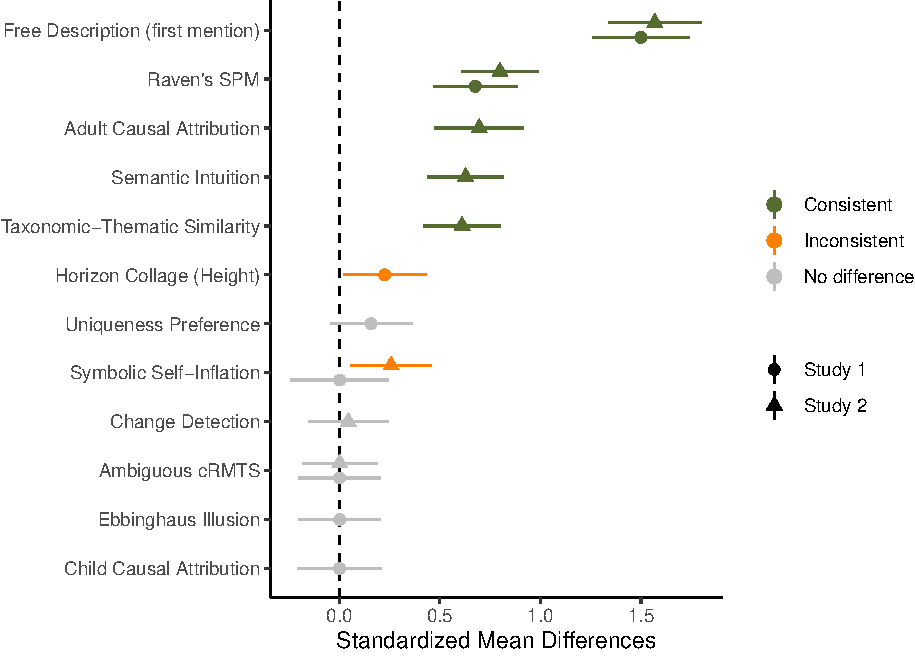
\includegraphics{CCRR_manuscript_files/figure-latex/es-plot-1.pdf}
\caption{\label{fig:es-plot}Forest plot of effect sizes (standardized mean difference) for each task across both experiments. Point shape shows experiment number and color indicates whether effects were consistent with prior literature.}
\end{figure}

Across our two experiments, we saw consistent and generally large differences (SMD \textgreater{} 0.6) in Free Description, Raven's SPM, Adult Causal Attribution, Semantic Intuition, and Taxonomic-Thematic Similarity tasks. Aside from Raven's SPM, all of these tasks have in common that they are deliberative linguistic tasks that tapped into relatively high-level cognitive constructs. In contrast, we observed effect sizes close to zero for our more aesthetic and perceptual tasks (Change Detection, Ebbinghaus Illusion, and Horizon Collage). We also observed little consistent difference in four other tasks (Ambiguous cRMTS, Symbolic Self-Inflation, Uniqueness Preference, and Child Causal Attribution), perhaps for reasons idiosyncratic to each. We return to the broader question of generalization across task types in the General Discussion.

We conducted three additional exploratory analyses to consolidate results from the two experiments. First, we assessed the reliability of the tasks that included multiple trials. Second, we examined whether there was shared variance between tasks. Finally, we examined how explicit cultural identities and demographic factors relate to task performance.

\hypertarget{reliability-assessment}{%
\subsection{Reliability assessment}\label{reliability-assessment}}

\begin{figure}
\centering
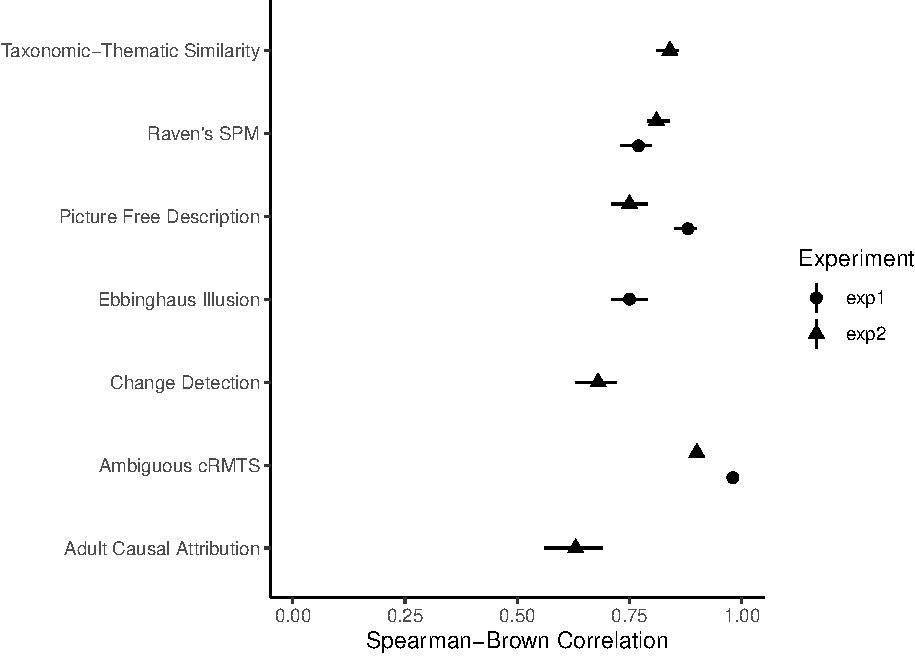
\includegraphics{CCRR_manuscript_files/figure-latex/reliability-1.pdf}
\caption{\label{fig:reliability}Spearman-Brown adjusted reliabilities for tasks with four or more trials. Point shape shows experiment number. Error bars show 95\% confidence intervals.}
\end{figure}

One question motivating our work was whether the individual tasks we used were reliable enough -- had low enough measurement error -- to be used for further investigation of individual differences. The gold standard for evaluating whether a task yields stable within-person measurements is test-retest reliability (simply because test-retest gives a direct estimate of stability over time), but this method was outside the scope of our study. Instead, we used a split-half approach, asking whether participants' answers on individual questions relate to one another. Specifically, we used a permutation-based split half approach (Parsons, 2021) in which we made 5000 random splits of items into two simulated ``halves'' and then computed the within-person correlation between scores on these two halves, averaging across simulated runs. To estimate the reliability of the full-length instrument, we used the Spearman-Brown ``prophecy'' formula.

Since the split-half approach is only suitable for tasks with multiple trials, we removed tasks with fewer than four trials from the analysis. For tasks with more than one condition, we focused on the condition that was predicted to show cultural differences (i.e., the Illusion context in the Ebbinghaus Illusion; situational factors in Adult Causal Attribution; background change scenes in Change Detection).

Figure \ref{fig:reliability} shows the corrected split-half reliabilities for all tasks in both of our experiments. Overall, the reliabilities were acceptable (all Spearman-Brown Correlations \textgreater{} 0.6). We further investigated whether there was cultural variation in the reliability of tasks. For most tasks, the reliabilities were relatively similar (within 0.1 of one another), but there were three tasks where reliability was lower for US participants than Chinese participants: Change Detection (US - CN = -0.19), Adult Causal Attribution (US - CN = -0.33), Free Description in Experiment 1 (US - CN = -0.23).

\hypertarget{relations-between-individual-tasks}{%
\subsection{Relations between individual tasks}\label{relations-between-individual-tasks}}

One (perhaps simplistic) interpretation of the prior literature on cultural variation is that there is a general tendency toward holistic or analytic reasoning that varies across cultures and explains variation in tasks. This single dimension might correspond to broad (or focused) attention and contextualized, relational reasoning (or an emphasis on focal people or objects). As a first step towards investigating this interpretation, we explored whether there was a single dimension of individual variation in our data that corresponded to this general axis of cross-cultural difference. Because some data was missing, largely due to task-related exclusions, we treated the missing data using two approaches: listwise deletion and imputation with means. These approaches yielded comparable results, so here we report correlations from listwise deletion.

Correlations between task scores were quite low on average, suggesting limited support for a single factor explanation. Across both experiments, the largest absolute magnitude of correlations observed were -0.29 (Taxonomic-Thematic Similarity and Adult Causal Attribution in Experiment 2), -0.28 (Free Description and Raven's SPM in Experiment 2), and -0.24 (Adult Causal Attribution and Free Description in Experiment 2). All other correlations were between -0.23 and 0.23. Hence, the amount of shared variation between tasks was quite limited and our attempts at exploratory factor analysis discovered structures with many distinct factors and very low loading on the first factor.

We also applied the same correlation analysis within each culture. Again, we found limited correlations between tasks. This pattern replicated the findings from a previous work showing negligible relationships among a battery of tasks that revealed cultural differences (Na et al., 2010) (See Appendix C).

\hypertarget{demographic-variation-and-explicit-measures-of-cultural-identity}{%
\subsection{Demographic variation and explicit measures of cultural identity}\label{demographic-variation-and-explicit-measures-of-cultural-identity}}

As a final exploratory analysis, we asked whether demographic variation or variation in cultural identity predicted responding in our tasks. Our approach to these questions was to fit a set of exploratory regression models for each task, predicting task scores as a function of an individual scale and its interaction with culture. This approach allowed us to explore both within- and between-culture effects in a single model. Our predictors were 1) the summed score for our global/local cultural identity and consumption measures (with local items reverse-scored, such that higher scores represent more global identities and consumption patterns); 2) geographic information about where participants grew up Markus \& Conner (2014); and 3) a range of demographic factors, including age, gender identity, residential mobility, number of international experiences, maternal education level, and subjective socioeconomic status as measured by the MacArthur Ladder (Adler et al., 2000).

\hypertarget{task-performance-and-global-identity}{%
\subsubsection{Task performance and global identity}\label{task-performance-and-global-identity}}

We fit models predicting task performance based on culture and its interaction with global (vs local) identity for tasks in Experiment 2 (we did not collect these scales in Experiment 1). Two of these relationships were statistically significant at .01 \textless{} p \textless{} .05 (Adult Causal Attribution: \emph{p} = 0.05; Taxonomic-Thematic Similarity: \emph{p} = 0.04) but neither of these relationships survived Bonferroni correction for multiple comparisons.

\hypertarget{task-performance-and-geographic-origin}{%
\subsubsection{Task performance and geographic origin}\label{task-performance-and-geographic-origin}}

We next considered whether regions within each country were meaningful predictors of task performance. We fit models predicting task performance based on the regions that participants reported growing up in. For China, provinces were categorized as rice-cultivating regions or wheat-cultivating regions based on Talhelm et al. (2014). For the US, states were categorized based on either the coastal locations (West Coast, East Coast, and Inland) or broad geographic locations (West, South, Northeast, Midwest), following the categorization reported in Carstensen, Saponaro, Frank, and Walker (2022).

5 out of the 48 models we ran showed statistically significant relationships between regions and task performance. In Experiment 1, US coastal location was a significant predictor for the Free Description task. Participants who grew up in Inland regions (\emph{N} = 54) or on the East Coast (\emph{N} = 27) were more likely to mention the focal object first when describing the pictures than participants who grew up on the West Coast (\emph{N} = 84; Inland: \emph{p} = 0.02; East Coast: \emph{p} = 0.05). In Experiment 2, both coastal location and broad geographic location were significant predictors for Raven's SPM, with participants from the East Coast (\emph{N} = 89) and Inland regions (\emph{N} = 159) scoring higher than participants from the West Coast (\emph{N} = 46; Inland: \emph{p} \textless{} 0.01; East Coast: \emph{p} = 0.05), and participants from the Midwest (\emph{N} = 78) and South (\emph{N} = 94) scoring higher than participants from the West (\emph{N} = 59; Midwest: \emph{p} \textless{} 0.01; South: \emph{p} = 0.04). In addition, both region categories predicted performance in Change Detection. East Coast participants (\emph{N} = 75) took longer to respond than West Coast (\emph{N} = 42) participants (\emph{p} = 0.02), and Northeastern participants (\emph{N} = 52) took longer to respond than participants who grew up in the West (\emph{N} = 52; \emph{p} \textless{} 0.01). However, none of these relationships survived Bonferroni correction.

\hypertarget{basic-demographic-effects}{%
\subsubsection{Basic demographic effects}\label{basic-demographic-effects}}

We fit 192 exploratory regression models to see if basic demographic factors could predict task performance. The demographic factors we explored were age, gender identity, residential mobility, number of international experiences, maternal education level, and subjective socioeconomic status as measured by the MacArthur Ladder (Adler et al., 2000). 26 were statistically significant, but only one model survived Bonferroni correction. Change detection was predicted by age in the US sample, with older participants taking longer to respond than younger participants (adjusted \emph{p} \textless{} 0.01). Given some of the models could be considered as conceptual replications of previous work, we reported selected models with significant uncorrected results in Appendix D.

\hypertarget{general-discussion}{%
\section{General Discussion}\label{general-discussion}}

The world's cultures are strikingly different, and psychologists have long sought to measure and characterize this variation, with differences between Western and East Asian cultures as a case study of particular interest. These efforts have given rise to a rich literature documenting cultural differences in a wide range of psychological tasks. Across two experiments, we selected a collection of tasks that had previously been shown to yield differences between Western and East Asian samples and replicated them with two relatively large online samples of participants from the US and China. In this discussion, we first consider the limitations of our study since these contextualize the remainder of our conclusions. Next, we consider the interpretation of our results within individual tasks. We end the discussion with a summary of the key findings of this work.

\hypertarget{general-limitations}{%
\subsection{General Limitations}\label{general-limitations}}

As discussed above and in the introduction, we did not design our experiments to replicate prior work directly, and hence one important limitation of our work is simply that it cannot be used as a test of the reliability of prior findings. Instead, our measures provide estimates of US-China differences on a range of constructs, specifically for online convenience samples. These estimates are likely biased downward -- towards the null hypothesis of no difference between cultures -- by several features of our experimental design.

Online experiments (especially grouped into a long battery as ours were) likely receive slightly less attention than in-person studies, though overall these effects have tended to be small in US samples (Buhrmester, Kwang, \& Gosling, 2016). Contra this concern, however, participants did perform relatively accurately on those tasks that had correct answers (e.g., Raven's SPM, the Ebbinghaus Illusion), and in our exploratory analysis, we found relatively high reliabilities on all tasks. Further, our pre-registered exclusion criteria removed participants who performed poorly. Thus, we do not believe that participants were inattentive overall.

One might also be concerned about the reaction time measures (e.g.~Ebbinghaus Illusion and Change Detection) collected through the online experiment. Due to variations in individual participants' hardware and internet conditions, the reaction times collected could potentially be more variable than those from in-person experiment. However, the validity of online reaction time measure has been evaluated and compared against in-person data across many different classic cognitive psychology tasks such as the Stroop task and the Flanker task. Across many tasks that require precise reaction time measures, online replications were qualitatively identical to the in-person version of the task (Crump, McDonnell, \& Gureckis, 2013). Moreover, some works have also evaluated the accuracy and reliabiltiy of jsPsych, the JavaScript library that we used (Anwyl-Irvine, Dalmaijer, Hodges, \& Evershed, 2021; Pinet et al., 2017). The consensus is that reaction time measures collected through jsPsych is reliable and accurate. Therefore, there is no reason to believe that the variability in our online reaction time measure deviated significantly from the in-person version of the reaction time task.

Another limitation of our estimates of US-China differences comes from variation in our sampling strategy between cultures. In Experiment 1, we used the same snowball sampling procedure, but this procedure may have yielded different samples due to differences in social networks or norms about sharing study information across cultures. In Experiment 2, because the platform we used to recruit US participants (Prolific) was not accessible in China, we used a different platform to recruit Chinese participants (Naodao). Prolific and Naodao have different levels of popularity and different participant pools, resulting in some asymmetry between the US and Chinese samples. Despite these differences between samples both across and within experiments, we do not see indications that our estimates were dramatically biased by our sampling decisions. First, our results were largely comparable in the tasks that were included in both experiments (e.g.~Picture Free Description; Raven's SPM; and Ambiguous cRMTS). Second, in our exploratory analyses we did not find strong associations between participant demographics and cross-cultural effects (with some small exceptions discussed in that section). Finally, we reran all of our preregistered analyses with an age-matched subset of U.S. participants in Experiment 2 and found our results were qualitatively identical.

Thus, while our samples are certainly not representative samples of US or Chinese national populations -- indeed to our knowledge, nearly all work to date has used convenience samples of one type or another -- they appear to yield stable cross-sample estimates that do not reflect large biases due to sampling strategy or demographics.

One of the main ways in which our samples may not have been representative is that they are likely to be more globalized than the population on average simply by being young (and thus less acculturated) and having access to a computer. Contra this concern, variation in local cultural identity did not strongly relate to variation in any of our tasks, but interestingly, we observed the strongest local identities (within our Chinese sample) among the youngest participants.

Last but not least, another difference between our experiments and previous work was the lack of an experimenter, and some of our tasks may be particularly sensitive to the presence of an experimenter. In a web experiment, participants are often isolated in front of their own computer. In contrast, in an in-person experiment, participants must interact with and perform the task in front of experimenters who are often from the same social group. Indeed, in the Uniqueness Preference pen choice task, cross-cultural differences are dependent on the presence of an experimenter (Yamagishi, Hashimoto, \& Schug, 2008). Our null results, obtained in the absence of an experimenter, can be seen as a conceptual replication of this work.

\hypertarget{task-specific-limitations}{%
\subsection{Task-specific Limitations}\label{task-specific-limitations}}

In addition to the general limitations discussed above, there are features of our experimental adaptations that may have affected performance in specific tasks. In this section, we highlight concerns about these issues and discuss their implications for interpreting the results of these tasks. See Table 2 for a summary of this task-specific discussion.

In the case of the Uniqueness Preference task, it is possible that adapting the task to an online format in which resource scarcity was not strictly real and task choices had no lasting effect (in the form of a new pen), may have trivialized the choice and undermined the incentive for prosocial, harmonious behavior or expression. This possibility is consistent with the chance responding we observed in both groups. Alternatively, our results could be seen as a conceptual replication of Yamagishi et al. (2008), who argue that differences in this task are moderated by the likelihood of evaluation, with no differences in pen choice observed in the absence of an experimenter.

The ambiguous developmental tasks, Ambiguous cRMTS and Child Causal Attribution, may have been too heavy-handed in their key manipulations; both were designed to highlight ambiguity for young children, but it may be that their explicit cues and repetitive instructions impressed this ambiguity too strongly for adult audiences, resulting in the adults' near-chance responding -- a reasonable response to such marked ambiguity. Cultural differences in causal reasoning and attribution may only manifest when the task design is age-appropriate. Consistent with this view, we did replicate previously attested differences in the Adult Causal Attribution task in Experiment 2, and other recent work has shown cross-cultural differences in causal attribution among 4- to 9-year-olds in Germany, Japan, and Ecuador using a design similar to the Child Causal Attribution task (Jurkat, Iza Simba, Hernández Chacón, Itakura, \& Kärtner, 2022).

Last but not least, variation within the broad cultural constructs of East Asia and the West could explain some of our findings, as a failure to extend previous work. Some of the tasks we included originally compared participants from other parts of East Asia and the West (e.g., Horizon Collage, Symbolic Self-Inflation, Change Detection; but c.f. Masuda, Ishii, and Kimura (2016) for an alternative account of mixed findings in change detection paradigms). For example, the Taxonomic-Thematic Similarity task replicated previously attested cross-cultural differences between the US and China both here and in other work (Le et al., 2021) but these differences failed to generalize to a US-Vietnam comparison, despite the cultural, historical, and geographic similarities between China and Vietnam. This variation suggests that similar psychological tendencies could be expressed differently under distinct sociocultural contexts and traditions, even across regions and countries that share many similarities. As another example, responding in the Horizon Collage could be modulated by variation between countries: Chinese and Japanese aesthetic traditions differ, so while Chinese and Japanese people may share a preference for highly contextualized information, this preference may be typically expressed through distinct visual techniques.

\hypertarget{conclusion}{%
\subsection{Conclusion}\label{conclusion}}

We conducted two experiments to examine the robustness of several classic experimental paradigms in cross-cultural psychology. Our results showed a heterogeneous pattern of successes and failures: some tasks yielded robust cultural differences across both experiments, while others showed no difference between cultures. We estimated the reliability of the tasks to be moderate, with only minor variation in reliability across cultures. We also explored the effects of a range of demographic variables, including explicit identification with global identity, regional differences within cultures, and several demographic characteristics. All of these had minimal relation to task performance.

Our goal here was not to perform direct replications that would shed light on the replicability of specific findings. Instead, since our methods, administration medium, sample, and analytic approach differed from the prior literature, our hope was to examine the robustness of these paradigms as a method for measuring US-China differences in an online context. Our work has several strengths relative to the prior literature, including larger samples of participants from the US and China, two broad groups of tasks implemented openly online (and reusable by future researchers), and a preregistered analysis plan that allows for the unbiased estimation of cross-cultural effects. In sum, we hope that our work here provides a foundation for future studies that seek to establish a robust and replicable science of cross-cultural difference.

\begin{landscape}
    \begin{longtable}{p{3cm}p{10cm}p{8cm}}\\
    \caption{Differences between our tasks, the original refernce tasks, and speculation about how these differences may have impacted our results.}\\
        \hline
        \bf{Task Name} & \bf{Difference between the current and original version} & \bf{Speculative reasons} \\
        \hline
        Ambiguous causal Relational Match-To-Sample (cRMTS) & 
        \begin{itemize}
        \item Age: The original experiment was conducted with young children; the current experiment was conducted with adults (but cf. Goddu, Sullivan, \& Walker (2021) for non-chance adult performance in a very similar paradigm).
        \item Test Format: The original experiment was conducted in person with physical stimuli and live experimenters; the current experiment was conducted through web-based interfaces with animation. 
        \end{itemize}&  
        \begin{itemize}
        \item The relation between objects might have been less salient when the stimuli were presented as schematic animation.
     \item Adults may have been overall less engaged with the tasks and paid less attention to the causal properties of the object pairs.
    \end{itemize}\\

Ebbinghaus Illusion & 
    \begin{itemize}
        \item Age: The original study was conducted with young children; the current experiment was conducted with adults.
        \item Culture: The original experiment compared Japanese participants with Canadian participants; the current experiment compared Chinese participants with U.S. participants."
    \end{itemize} & 
    \begin{itemize}
        \item Adults in both cultures reached ceiling performance. 
        \item U.S. and Chinese participants may differ in visual context sensitivity compared to Canadian and Japanese participants.
    \end{itemize} \\

Horizon Collage  & 
    \begin{itemize}
        \item Age: The original experiment was conducted with young children; the current experiment was conducted with adults.
        \item Test Format: The original experiment was conducted in person with paper and collage stickers; the current experiment was conducted through web-based interfaces.
        \item Culture: The original experiment compared Japanese participants with Canadian participants; the current experiment compared Chinese participants with U.S. participants.
    \end{itemize} &
    \begin{itemize}
        \item The task might have been too trivial for adults to engage with properly. 
        \item The saliency of horizon height is diminished by the drag-and-drop online interface.
    \end{itemize}
    \\

Symbolic Self-Inflation (Family version and Friends version) & 
    \begin{itemize}
        \item Test Format: The original experiment was conducted in person with pen and paper; the current experiment was conducted through web-based interfaces.
        \item Test Prompt (Family version): The original experiment asked the participants to draw their close social network; the current experiment asked the participants to draw their family members or friends growing up.
    \end{itemize} & 
    \begin{itemize}
        \item The online interface might have altered participants’ drawing process, making it more difficult to implicitly represent the symbolic meaning of the circle size.
    \end{itemize}
     \\

Uniqueness Preference & 
    \begin{itemize}
        \item Test Format: The original experiment was conducted in person; the current experiment was conducted through web-based interfaces.
        \item Stimulus: The original experiment gave away physical pens to keep; the current experiment asked participants to select virtual stickers.
        \item Test Context: The original experiment prompted participants to make their pen selection after completing a questionnaire indicating their aesthetic preference for abstract art with unique or repeating shapes.
    \end{itemize}   & 
    \begin{itemize}
        \item The choice between virtual stickers is less meaningful than between real pens.
        \item The presence of a live experimenter might increase the social pressure on participants, causing them to consider the cultural perception of their choice.
        \item This richer context may have prompted more careful consideration of the key prompt.
    \end{itemize} \\

Child Causal Attribution & 
    \begin{itemize}
        \item Age: The original experiment was conducted with young children; the current experiment was conducted with adults.
    \end{itemize}
& \begin{itemize}
    \item Adults may have failed to engage deeply in causal reasoning because the story is too simplistic.
\end{itemize} \\

Change Detection & 
\begin{itemize}
    \item Test Format: The original experiment was conducted in person; the current experiment was conducted through web-based interfaces.
\end{itemize} & 
\begin{itemize}
    \item The in-lab setting might facilitate participants’ performance by making them pay more attention to the computer screen. 
\end{itemize}\\

    \hline
    \end{longtable}


\end{landscape}

\setlength{\parindent}{-0.5in}
\setlength{\leftskip}{0.5in}

\newpage

\hypertarget{references}{%
\section{References}\label{references}}

\hypertarget{refs}{}
\begin{CSLReferences}{1}{0}
\leavevmode\vadjust pre{\hypertarget{ref-adler2000relationship}{}}%
Adler, N. E., Epel, E. S., Castellazzo, G., \& Ickovics, J. R. (2000). Relationship of subjective and objective social status with psychological and physiological functioning. \emph{Health Psychology}, \emph{19}(6), 586.

\leavevmode\vadjust pre{\hypertarget{ref-anwyl2021realistic}{}}%
Anwyl-Irvine, A., Dalmaijer, E. S., Hodges, N., \& Evershed, J. K. (2021). Realistic precision and accuracy of online experiment platforms, web browsers, and devices. \emph{Behavior Research Methods}, \emph{53}, 1407--1425.

\leavevmode\vadjust pre{\hypertarget{ref-arnett2016neglected}{}}%
Arnett, J. J. (2016). The neglected 95\%: Why american psychology needs to become less american.

\leavevmode\vadjust pre{\hypertarget{ref-barr2013random}{}}%
Barr, D. J., Levy, R., Scheepers, C., \& Tily, H. J. (2013). Random effects structure for confirmatory hypothesis testing: Keep it maximal. \emph{Journal of Memory and Language}, \emph{68}(3), 255--278.

\leavevmode\vadjust pre{\hypertarget{ref-blouin2004difference}{}}%
Blouin, D. C., \& Riopelle, A. J. (2004). The difference between t and z and the difference it makes. \emph{J of Gen Psych}, \emph{131}(1), 77--84.

\leavevmode\vadjust pre{\hypertarget{ref-buhrmester2016amazon}{}}%
Buhrmester, M., Kwang, T., \& Gosling, S. D. (2016). Amazon's mechanical turk: A new source of inexpensive, yet high-quality data?

\leavevmode\vadjust pre{\hypertarget{ref-carstensen2022bridging}{}}%
Carstensen, A., Saponaro, C., Frank, M. C., \& Walker, C. M. (2022). Bridging cultural and cognitive perspectives on similarity reasoning. In \emph{Proceedings of the annual meeting of the cognitive science society} (Vol. 44).

\leavevmode\vadjust pre{\hypertarget{ref-carstensen2019context}{}}%
Carstensen, A., Zhang, J., Heyman, G. D., Fu, G., Lee, K., \& Walker, C. M. (2019). Context shapes early diversity in abstract thought. \emph{PNAS}, \emph{116}(28), 13891--13896.

\leavevmode\vadjust pre{\hypertarget{ref-champely2018package}{}}%
Champely, S., Ekstrom, C., Dalgaard, P., Gill, J., Weibelzahl, S., Anandkumar, A., \ldots{} De Rosario, M. H. (2018). Package {``pwr.''} \emph{R Package Version}, \emph{1}(2).

\leavevmode\vadjust pre{\hypertarget{ref-chan2011english}{}}%
Chan, C. C., Tardif, T., Chen, J., Pulverman, R. B., Zhu, L., \& Meng, X. (2011). English-and chinese-learning infants map novel labels to objects and actions differently. \emph{Dev Psy}, \emph{47}(5), 1459.

\leavevmode\vadjust pre{\hypertarget{ref-cheng2020development}{}}%
Cheng, L. (2020). \emph{The development of cognitive styles among american and chinese children} (PhD thesis).

\leavevmode\vadjust pre{\hypertarget{ref-choi1999causal}{}}%
Choi, I., Nisbett, R. E., \& Norenzayan, A. (1999). Causal attribution across cultures. \emph{Psy Bull}, \emph{125}(1), 47.

\leavevmode\vadjust pre{\hypertarget{ref-chua2005cultural}{}}%
Chua, H. F., Boland, J. E., \& Nisbett, R. E. (2005). Cultural variation in eye movements during scene perception. \emph{PNAS}, \emph{102}(35), 12629--12633.

\leavevmode\vadjust pre{\hypertarget{ref-cleveland2007acculturaton}{}}%
Cleveland, M., \& Laroche, M. (2007). Acculturaton to the global consumer culture: Scale development and research paradigm. \emph{Journal of Business Research}, \emph{60}(3), 249--259.

\leavevmode\vadjust pre{\hypertarget{ref-cleveland2015intersection}{}}%
Cleveland, M., Laroche, M., \& Takahashi, I. (2015). The intersection of global consumer culture and national identity and the effect on japanese consumer behavior. \emph{Journal of International Consumer Marketing}, \emph{27}(5), 364--387.

\leavevmode\vadjust pre{\hypertarget{ref-corriveau2017cultural}{}}%
Corriveau, K. H., DiYanni, C. J., Clegg, J. M., Min, G., Chin, J., \& Nasrini, J. (2017). Cultural differences in the imitation and transmission of inefficient actions. \emph{J Exp Child Psy}, \emph{161}, 1--18.

\leavevmode\vadjust pre{\hypertarget{ref-crump2013evaluating}{}}%
Crump, M. J., McDonnell, J. V., \& Gureckis, T. M. (2013). Evaluating amazon's mechanical turk as a tool for experimental behavioral research. \emph{PloS One}, \emph{8}(3), e57410.

\leavevmode\vadjust pre{\hypertarget{ref-de2015jspsych}{}}%
De Leeuw, J. R. (2015). jsPsych: A JavaScript library for creating behavioral experiments in a web browser. \emph{Behavior Research Methods}, \emph{47}(1), 1--12.

\leavevmode\vadjust pre{\hypertarget{ref-diyanni2015role}{}}%
DiYanni, C. J., Corriveau, K. H., Kurkul, K., Nasrini, J., \& Nini, D. (2015). The role of consensus and culture in children's imitation of inefficient actions. \emph{J Exp Child Psy}, \emph{137}, 99--110.

\leavevmode\vadjust pre{\hypertarget{ref-doherty2008context}{}}%
Doherty, M. J., Tsuji, H., \& Phillips, W. A. (2008). The context sensitivity of visual size perception varies across cultures. \emph{Perception}, \emph{37}(9), 1426--1433.

\leavevmode\vadjust pre{\hypertarget{ref-duffy2009development}{}}%
Duffy, S., Toriyama, R., Itakura, S., \& Kitayama, S. (2009). Development of cultural strategies of attention in {N}orth {A}merican and {J}apanese children. \emph{J Exp Child Psy}, \emph{102}(3), 351--359.

\leavevmode\vadjust pre{\hypertarget{ref-flake2020measurement}{}}%
Flake, J. K., \& Fried, E. I. (2020). Measurement schmeasurement: Questionable measurement practices and how to avoid them. \emph{Advances in Methods and Practices in Psychological Science}, \emph{3}(4), 456--465.

\leavevmode\vadjust pre{\hypertarget{ref-goddu2021toddlers}{}}%
Goddu, M. K., Sullivan, J. N., \& Walker, C. M. (2021). Toddlers learn and flexibly apply multiple possibilities. \emph{Child Development}, \emph{92}(6), 2244--2251.

\leavevmode\vadjust pre{\hypertarget{ref-green2016simr}{}}%
Green, P., \& MacLeod, C. J. (2016). SIMR: An r package for power analysis of generalized linear mixed models by simulation. \emph{Methods in Ecology and Evolution}, \emph{7}(4), 493--498.

\leavevmode\vadjust pre{\hypertarget{ref-hauser1994measuring}{}}%
Hauser, R. M. (1994). Measuring socioeconomic status in studies of child development. \emph{Child Development}, \emph{65}(6), 1541--1545.

\leavevmode\vadjust pre{\hypertarget{ref-henrich2010weirdest}{}}%
Henrich, J., Heine, S. J., \& Norenzayan, A. (2010). The weirdest people in the world? \emph{Behav Brain Sci}, \emph{33}(2-3), 61--83.

\leavevmode\vadjust pre{\hypertarget{ref-hoff2005socioeconomic}{}}%
Hoff, E., \& Tian, C. (2005). Socioeconomic status and cultural influences on language. \emph{Journal of Communication Disorders}, \emph{38}(4), 271--278.

\leavevmode\vadjust pre{\hypertarget{ref-imada2013east}{}}%
Imada, T., Carlson, S. M., \& Itakura, S. (2013). East--west cultural differences in context-sensitivity are evident in early childhood. \emph{Dev Sci}, \emph{16}(2), 198--208.

\leavevmode\vadjust pre{\hypertarget{ref-ishii2020residential}{}}%
Ishii, K., Komiya, A., \& Oishi, S. (2020). Residential mobility fosters sensitivity to the disappearance of happiness. \emph{International Journal of Psychology}, \emph{55}(4), 577--584.

\leavevmode\vadjust pre{\hypertarget{ref-ji2001culture}{}}%
Ji, L.-J., Nisbett, R. E., \& Su, Y. (2001). Culture, change, and prediction. \emph{Psych Sci}, \emph{12}(6), 450--456.

\leavevmode\vadjust pre{\hypertarget{ref-ji2000culture}{}}%
Ji, L.-J., Peng, K., \& Nisbett, R. E. (2000). Culture, control, and perception of relationships in the environment. \emph{JPSP}, \emph{78}(5), 943.

\leavevmode\vadjust pre{\hypertarget{ref-ji2004culture}{}}%
Ji, L.-J., Zhang, Z., \& Nisbett, R. E. (2004). Is it culture or is it language? \emph{JPSP}, \emph{87}(1), 57.

\leavevmode\vadjust pre{\hypertarget{ref-jurkat2022cultural}{}}%
Jurkat, S., Iza Simba, N. B., Hernández Chacón, L., Itakura, S., \& Kärtner, J. (2022). Cultural similarities and differences in explaining others' behavior in 4-to 9-year-old children from three cultural contexts. \emph{Journal of Cross-Cultural Psychology}, 00220221221098423.

\leavevmode\vadjust pre{\hypertarget{ref-kim1999deviance}{}}%
Kim, H., \& Markus, H. R. (1999). Deviance or uniqueness, harmony or conformity? A cultural analysis. \emph{JPSP}, \emph{77}(4), 785.

\leavevmode\vadjust pre{\hypertarget{ref-kitayama2009cultural}{}}%
Kitayama, S., Park, H., Sevincer, A. T., Karasawa, M., \& Uskul, A. K. (2009). A cultural task analysis of implicit independence. \emph{JPSP}, \emph{97}(2), 236.

\leavevmode\vadjust pre{\hypertarget{ref-kuwabara2012cross}{}}%
Kuwabara, M., \& Smith, L. B. (2012). Cross-cultural differences in cognitive development: Attention to relations and objects. \emph{J Exp Child Psy}, \emph{113}(1), 20--35.

\leavevmode\vadjust pre{\hypertarget{ref-kwan1997pancultural}{}}%
Kwan, V. S., Bond, M. H., \& Singelis, T. M. (1997). Pancultural explanations for life satisfaction: Adding relationship harmony to self-esteem. \emph{JPSP}, \emph{73}(5), 1038.

\leavevmode\vadjust pre{\hypertarget{ref-le2021}{}}%
Le, K., Frank, M., \& Carstensen, Alex. (2021). \emph{Is it language or is it culture? Re-examining cross-cultural similarity judgments using lexical co-occurrence} (Undergraduate Honors Theses). Stanford University.

\leavevmode\vadjust pre{\hypertarget{ref-li2018name}{}}%
Li, J., Liu, L., Chalmers, E., \& Snedeker, J. (2018). What is in a name?: The development of cross-cultural differences in referential intuitions. \emph{Cognition}, \emph{171}, 108--111.

\leavevmode\vadjust pre{\hypertarget{ref-liang2012effect}{}}%
Liang, B., \& He, Y. (2012). The effect of culture on consumer choice: The need for conformity vs. The need for uniqueness. \emph{Int J of Consum Stu}, \emph{36}(3), 352--359.

\leavevmode\vadjust pre{\hypertarget{ref-machery2020replication}{}}%
Machery, E. (2020). What is a replication? \emph{Philosophy of Science}, \emph{87}(4), 545--567.

\leavevmode\vadjust pre{\hypertarget{ref-markus2014clash}{}}%
Markus, H. R., \& Conner, A. (2014). \emph{Clash!: How to thrive in a multicultural world}. Penguin.

\leavevmode\vadjust pre{\hypertarget{ref-markus1992and}{}}%
Markus, H. R., \& Kitayama, S. (1992). The what, why and how of cultural psychology: A review of shweder's thinking through cultures. \emph{Psychological Inquiry}, \emph{3}(4), 357--364.

\leavevmode\vadjust pre{\hypertarget{ref-markus2010cultures}{}}%
Markus, H. R., \& Kitayama, S. (2010). Cultures and selves: A cycle of mutual constitution. \emph{Perspectives on Psychological Science}, \emph{5}(4), 420--430.

\leavevmode\vadjust pre{\hypertarget{ref-masuda2016does}{}}%
Masuda, T., Ishii, K., \& Kimura, J. (2016). When does the culturally dominant mode of attention appear or disappear? Comparing patterns of eye movement during the visual flicker task between european canadians and japanese. \emph{Journal of Cross-Cultural Psychology}, \emph{47}(7), 997--1014.

\leavevmode\vadjust pre{\hypertarget{ref-masuda2006culture}{}}%
Masuda, T., \& Nisbett, R. E. (2006). Culture and change blindness. \emph{Cognitive Science}, \emph{30}(2), 381--399.

\leavevmode\vadjust pre{\hypertarget{ref-mercier2012use}{}}%
Mercier, H., Yama, H., Kawasaki, Y., Adachi, K., \& Van der Henst, J.-B. (2012). Is the use of averaging in advice taking modulated by culture? \emph{J Cog \& Culture}, \emph{12}(1-2), 1--16.

\leavevmode\vadjust pre{\hypertarget{ref-mercier2015easterners}{}}%
Mercier, H., Zhang, J., Qu, Y., Lu, P., \& Van der Henst, J.-B. (2015). Do easterners and westerners treat contradiction differently? \emph{J Cog \& Culture}, \emph{15}(1-2), 45--63.

\leavevmode\vadjust pre{\hypertarget{ref-miyamoto2018culture}{}}%
Miyamoto, Y., Yoo, J., Levine, C. S., Park, J., Boylan, J. M., Sims, T., et al.others. (2018). Culture and social hierarchy: Self-and other-oriented correlates of socioeconomic status across cultures. \emph{Journal of Personality and Social Psychology}, \emph{115}(3), 427.

\leavevmode\vadjust pre{\hypertarget{ref-moriguchi2012cultural}{}}%
Moriguchi, Y., Evans, A. D., Hiraki, K., Itakura, S., \& Lee, K. (2012). Cultural differences in the development of cognitive shifting. \emph{J Exp Child Psy}, \emph{111}(2), 156--163.

\leavevmode\vadjust pre{\hypertarget{ref-morris1995causal}{}}%
Morris, M. W., Nisbett, R. E., \& Peng, K. (1995). Causal attribution across domains and cultures.

\leavevmode\vadjust pre{\hypertarget{ref-morris1994culture}{}}%
Morris, M. W., \& Peng, K. (1994). Culture and cause: American and chinese attributions for social and physical events. \emph{JPSP}, \emph{67}(6), 949.

\leavevmode\vadjust pre{\hypertarget{ref-muthukrishna2020beyond}{}}%
Muthukrishna, M., Bell, A. V., Henrich, J., Curtin, C. M., Gedranovich, A., McInerney, J., \& Thue, B. (2020). Beyond WEIRD psychology: Measuring and mapping scales of cultural and psychological distance. \emph{Psych Sci}, \emph{31}(6), 678--701.

\leavevmode\vadjust pre{\hypertarget{ref-na2020culture}{}}%
Na, J., Grossmann, I., Varnum, M. E., Karasawa, M., Cho, Y., Kitayama, S., \& Nisbett, R. E. (2020). Culture and personality revisited: Behavioral profiles and within-person stability in interdependent (vs. Independent) social orientation and holistic (vs. Analytic) cognitive style. \emph{Journal of Personality}, \emph{88}(5), 908--924.

\leavevmode\vadjust pre{\hypertarget{ref-na2010cultural}{}}%
Na, J., Grossmann, I., Varnum, M. E., Kitayama, S., Gonzalez, R., \& Nisbett, R. E. (2010). Cultural differences are not always reducible to individual differences. \emph{PNAS}, \emph{107}(14), 6192--6197.

\leavevmode\vadjust pre{\hypertarget{ref-nielsen2017persistent}{}}%
Nielsen, M., Haun, D., Kärtner, J., \& Legare, C. H. (2017). The persistent sampling bias in developmental psychology: A call to action. \emph{J Exp Child Psy}, \emph{162}, 31--38.

\leavevmode\vadjust pre{\hypertarget{ref-nosek2020replication}{}}%
Nosek, B. A., \& Errington, T. M. (2020). What is replication? \emph{PLoS Biology}, \emph{18}(3), e3000691.

\leavevmode\vadjust pre{\hypertarget{ref-oishi2022socio}{}}%
Oishi, S., \& Tsang, S. (2022). The socio-ecological psychology of residential mobility. \emph{Journal of Consumer Psychology}, \emph{32}(3), 519--536.

\leavevmode\vadjust pre{\hypertarget{ref-open2015estimating}{}}%
Open Science Collaboration. (2015). Estimating the reproducibility of psychological science. \emph{Science}, \emph{349}(6251).

\leavevmode\vadjust pre{\hypertarget{ref-parsons2021splithalf}{}}%
Parsons, S. (2021). Splithalf: Robust estimates of split half reliability. \emph{Journal of Open Source Software}, \emph{6}(60), 3041.

\leavevmode\vadjust pre{\hypertarget{ref-pinet2017measuring}{}}%
Pinet, S., Zielinski, C., Mathôt, S., Dufau, S., Alario, F.-X., \& Longcamp, M. (2017). Measuring sequences of keystrokes with jsPsych: Reliability of response times and interkeystroke intervals. \emph{Behavior Research Methods}, \emph{49}, 1163--1176.

\leavevmode\vadjust pre{\hypertarget{ref-richland2010young}{}}%
Richland, L. E., Chan, T.-K., Morrison, R. G., \& Au, T. K.-F. (2010). Young children's analogical reasoning across cultures: Similarities and differences. \emph{J Exp Child Psy}, \emph{105}(1-2), 146--153.

\leavevmode\vadjust pre{\hypertarget{ref-sabbagh2006development}{}}%
Sabbagh, M. A., Xu, F., Carlson, S. M., Moses, L. J., \& Lee, K. (2006). The development of executive functioning and theory of mind: A comparison of chinese and US preschoolers. \emph{Psych Sci}, \emph{17}(1), 74--81.

\leavevmode\vadjust pre{\hypertarget{ref-seiver2013did}{}}%
Seiver, E., Gopnik, A., \& Goodman, N. D. (2013). Did she jump because she was the big sister or because the trampoline was safe? \emph{Child Dev}, \emph{84}(2), 443--454.

\leavevmode\vadjust pre{\hypertarget{ref-senzaki2014holistic}{}}%
Senzaki, S., Masuda, T., \& Nand, K. (2014). Holistic versus analytic expressions in artworks: Cross-cultural differences and similarities in drawings and collages by {C}anadian and {J}apanese school-age children. \emph{J Cross Cult Psy}, \emph{45}(8), 1297--1316.

\leavevmode\vadjust pre{\hypertarget{ref-simmons2011}{}}%
Simmons, J. P., Nelson, L. D., \& Simonsohn, U. (2011). False-positive psychology. \emph{Psych Sci}, \emph{22}(11), 1359--1366.

\leavevmode\vadjust pre{\hypertarget{ref-spencer2009dialectical}{}}%
Spencer-Rodgers, J., Boucher, H. C., Mori, S. C., Wang, L., \& Peng, K. (2009). The dialectical self-concept. \emph{Pers Soc Psy B}, \emph{35}(1), 29--44.

\leavevmode\vadjust pre{\hypertarget{ref-spencer2009cultural}{}}%
Spencer-Rodgers, J., Boucher, H. C., Peng, K., \& Wang, L. (2009). Cultural differences in self-verification. \emph{J Exp Soc Psy}, \emph{45}(4), 860--866.

\leavevmode\vadjust pre{\hypertarget{ref-spencer2007culture}{}}%
Spencer-Rodgers, J., Williams, M. J., Hamilton, D. L., Peng, K., \& Wang, L. (2007). Culture and group perception: Dispositional and stereotypic inferences about novel and national groups. \emph{JPSP}, \emph{93}(4), 525.

\leavevmode\vadjust pre{\hypertarget{ref-su2020analogical}{}}%
Su, S. (2020). \emph{Analogical reasoning in {C}hinese and {US} adults} (Master's thesis). Cornell University.

\leavevmode\vadjust pre{\hypertarget{ref-talhelm2014large}{}}%
Talhelm, T., Zhang, X., Oishi, S., Shimin, C., Duan, D., Lan, X., \& Kitayama, S. (2014). Large-scale psychological differences within {C}hina explained by rice versus wheat agriculture. \emph{Science}, \emph{344}(6184), 603--608.

\leavevmode\vadjust pre{\hypertarget{ref-tan2020chinese}{}}%
Tan, B. (2020). \emph{Chinese and US young children's executive function and its sociocultural antecedents} (PhD thesis). The University of Memphis.

\leavevmode\vadjust pre{\hypertarget{ref-tan2020association}{}}%
Tan, J. J., Kraus, M. W., Carpenter, N. C., \& Adler, N. E. (2020). The association between objective and subjective socioeconomic status and subjective well-being: A meta-analytic review. \emph{Psychological Bulletin}, \emph{146}(11), 970.

\leavevmode\vadjust pre{\hypertarget{ref-tardif1996nouns}{}}%
Tardif, T. (1996). Nouns are not always learned before verbs: Evidence from mandarin speakers' early vocabularies. \emph{Dev Psy}, \emph{32}(3), 492.

\leavevmode\vadjust pre{\hypertarget{ref-waxman2016early}{}}%
Waxman, S. R., Fu, X., Ferguson, B., Geraghty, K., Leddon, E., Liang, J., \& Zhao, M.-F. (2016). How early is infants' attention to objects and actions shaped by culture? New evidence from 24-month-olds raised in the US and china. \emph{Front Psy}, \emph{7}, 97.

\leavevmode\vadjust pre{\hypertarget{ref-westfall2014statistical}{}}%
Westfall, J., Kenny, D. A., \& Judd, C. M. (2014). Statistical power and optimal design in experiments in which samples of participants respond to samples of stimuli. \emph{Journal of Experimental Psychology: General}, \emph{143}(5), 2020.

\leavevmode\vadjust pre{\hypertarget{ref-yamagishi2008preferences}{}}%
Yamagishi, T., Hashimoto, H., \& Schug, J. (2008). Preferences versus strategies as explanations for culture-specific behavior. \emph{Psychological Science}, \emph{19}(6), 579--584.

\leavevmode\vadjust pre{\hypertarget{ref-zhou2008perceiving}{}}%
Zhou, J., Gotch, C., Zhou, Y., \& Liu, Z. (2008). Perceiving an object in its context---is the context cultural or perceptual? \emph{Journal of Vision}, \emph{8}(12), 2--2.

\leavevmode\vadjust pre{\hypertarget{ref-zwaan2018making}{}}%
Zwaan, R. A., Etz, A., Lucas, R. E., \& Donnellan, M. B. (2018). Making replication mainstream. \emph{Behavioral and Brain Sciences}, \emph{41}.

\end{CSLReferences}

\newpage

\newpage

\hypertarget{appendix-appendix}{%
\appendix}


\hypertarget{prospective-power-analysis}{%
\section{Prospective Power analysis}\label{prospective-power-analysis}}

We conducted two power analyses: a low assumption t-test power analysis and a high assumption linear mixed effects model power analysis. Under both power analysis frameworks, we showed that our sample sizes are well-powered to detect medium and larger effect sizes.

\hypertarget{low-assumption-t-test-power-analysis}{%
\subsection{Low assumption t-test power analysis}\label{low-assumption-t-test-power-analysis}}

In this framework, we assumed the cultural differences are evaluated with a simple t-test between two samples. We varied the hypothetical effect sizes of the cultural differences. This analysis was conducted using the \texttt{pwr} package (Champely et al., 2018).

\hypertarget{high-assumption-mixed-effects-linear-regression-power-analysis}{%
\subsection{High assumption mixed effects linear regression power analysis}\label{high-assumption-mixed-effects-linear-regression-power-analysis}}

Conducting prospective power analysis for mixed-effects linear regression requires more assumptions. Here we specify a simplified model to run the power simulation on. The model predicts a response with culture as the fixed effect, and subjects as the random intercepts. We assumed the fixed effect's intercept and slope as 0.1 and 0.5, respectively. We varied the effect sizes of the model by manipulating different residual standard deviation. We conducted this analysis in the \texttt{simr} package (Green \& MacLeod, 2016).

\begin{figure}
\centering
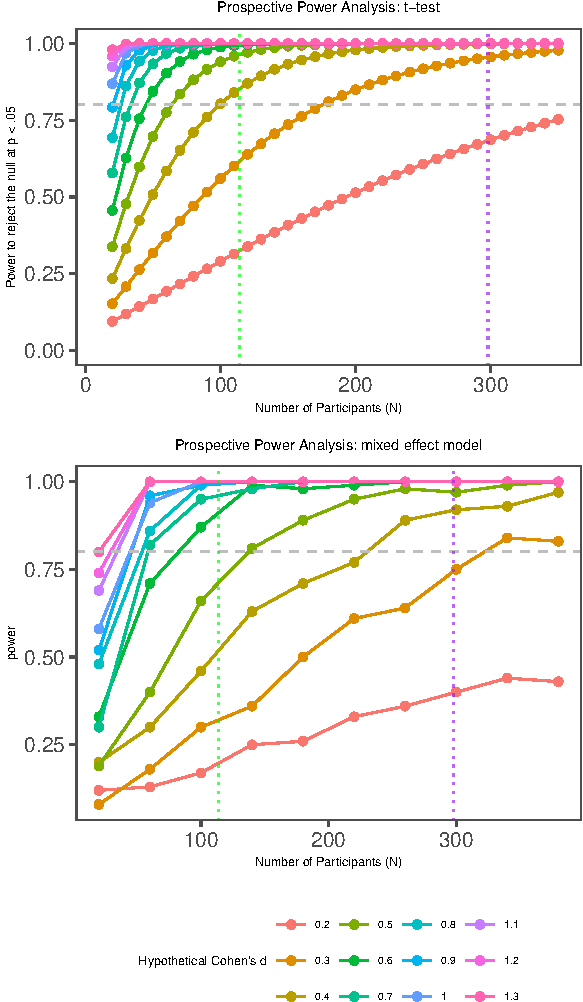
\includegraphics{CCRR_manuscript_files/figure-latex/unnamed-chunk-41-1.pdf}
\caption{\label{fig:unnamed-chunk-41}Simulation of power under different sample sizes and effect sizes. The top panel is under t-test assumptions, and the bottom panel is under linear mixed effect model assumptions. X-axis represents the number of particints in each condition. Y-axis represents the estimated power based on the effect sizes and the sample sizes. The horizontal gray dotted line on each plot represents 80\% power. The two vertical lines, green and purple, represents the minimum sample size and the maximum sample size in our study, respectively.}
\end{figure}

\hypertarget{additional-visualizations-for-task-results}{%
\section{Additional Visualizations for Task Results}\label{additional-visualizations-for-task-results}}

\hypertarget{free-description}{%
\subsection{Free Description}\label{free-description}}

One measure from the Picture Free Description task is the number of descriptive accounts directed at the focal objects versus the background objects. In Experiment 1, we found a main effect of culture, with U.S. participants providing more description overall. We also found an interaction effect between culture and description types, with U.S. participants providing more background descriptions than focal descriptions. This pattern was inconsistent with the results reported in Imada et al. (2013). However, we found a pattern consistent with the original findings in experiment 2: Chinese participants provided more descriptive accounts directed at the background objects than the focal objects relative to U.S. participants. We reported the descriptive and inferential statistics in the main text.

\begin{figure}
\centering
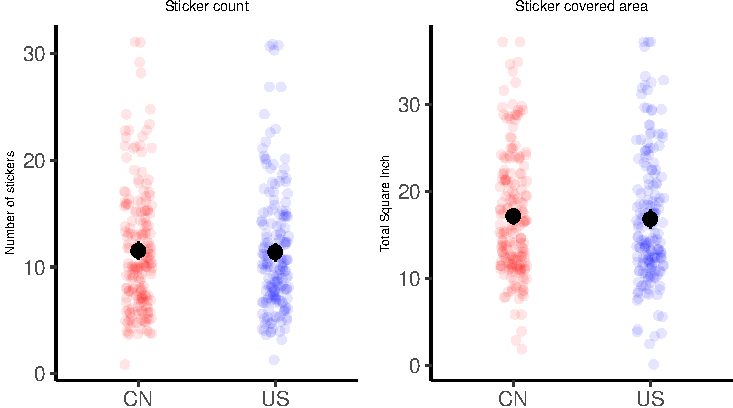
\includegraphics{CCRR_manuscript_files/figure-latex/unnamed-chunk-44-1.pdf}
\caption{\label{fig:unnamed-chunk-44}Results from the Picture Free Description task's descriptive accounts measures for experiment 1 and experiment 2 respectively. Each dot represents the number of descriptive accounts directed at either the focal object or the background object in each trial. Red indicates Chinese participants' responses, and blue indicates U.S. participants' responses. The black dots are the mean values for each group, with error bars showing 95\% confidence intervals}
\end{figure}

\hypertarget{horizon-collage-1}{%
\subsection{Horizon Collage}\label{horizon-collage-1}}

In Horizon Collage task, we included two other measures in addition to the height of horizon: the number of stickers and the total area that the stickers covered. Here we included the visualization for the latter two measures. Unlike Senzaki et al. (2014), we did not see any cultural difference in either measure. We reported the descriptive and inferential statistics in the main text.

\begin{figure}
\centering
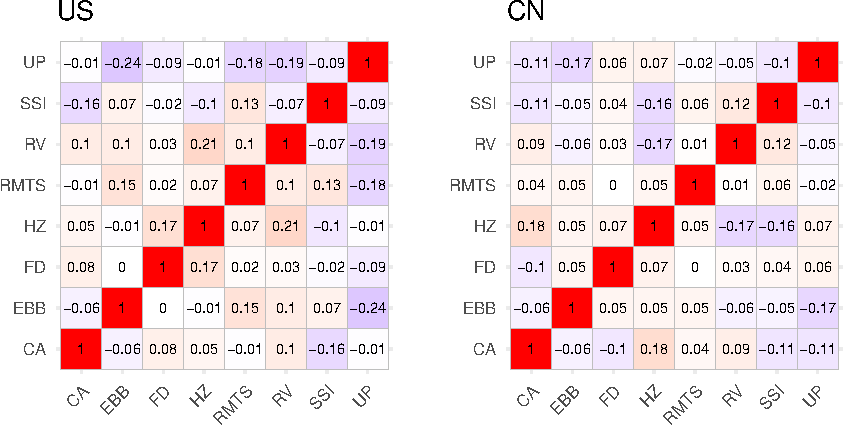
\includegraphics{CCRR_manuscript_files/figure-latex/unnamed-chunk-46-1.pdf}
\caption{\label{fig:unnamed-chunk-46}Results from the Horizon Collage task's sticker number and sticker covered area measures. Each dot represents one participant's response. Red indicates Chinese participants' responses, and blue indicates U.S. participants' responses. The black dots are the mean values for each group, with error bars showing 95\% confidence intervals}
\end{figure}

\hypertarget{within-culture-analysis-on-relationships-between-tasks.}{%
\section{Within-culture analysis on relationships between tasks.}\label{within-culture-analysis-on-relationships-between-tasks.}}

Na et al. (2010) found neglible correlations among a battery of tasks that revealed cultural differences within each culture. We found similar patterns in our data. Here we report four correlation matrices: US participants' correlation matrix is on the left, and Chinese participants' on the right. Each cell has a number indicating the correlation between the task marked on the column head and the task marked on the row head (Experiment 1: CA = Child Causal Attribution; EBB: Ebbinghaus Illusion; FD = Free Description; HZ = Horizon Collage; RMTS = Ambiguous cRMTS; RV = Raven's Progressive Matrices; SSI = Symbolic Self-Inflation; UP = Uniqueness Preference; Experiment 2: RMTS = Ambiguous cRMTS; RV = Raven's Progressive Matrices; FD = Free Description; CD = Change Detection; SSI = Symbolic Self-Inflation; CA = Causal Attribution; TTS = Taxonomic-Thematic Similarity; SeI = Semantic Intuition).

\hypertarget{experiment-1-1}{%
\subsection{Experiment 1}\label{experiment-1-1}}

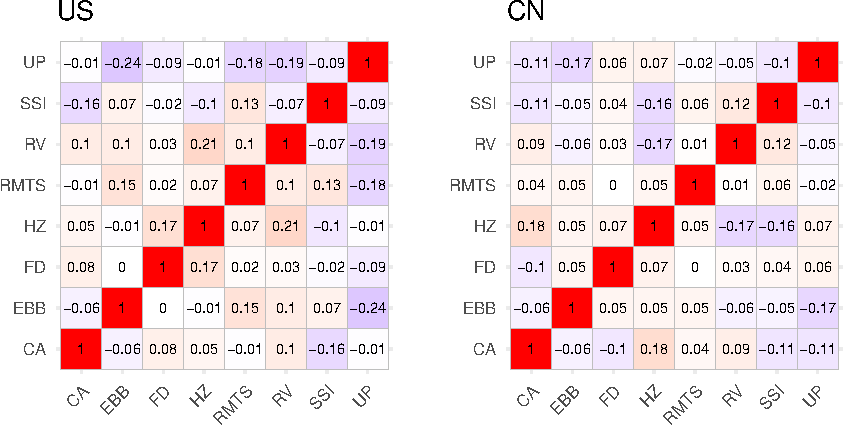
\includegraphics{CCRR_manuscript_files/figure-latex/unnamed-chunk-48-1.pdf}

\hypertarget{experiment-2-1}{%
\subsection{Experiment 2}\label{experiment-2-1}}

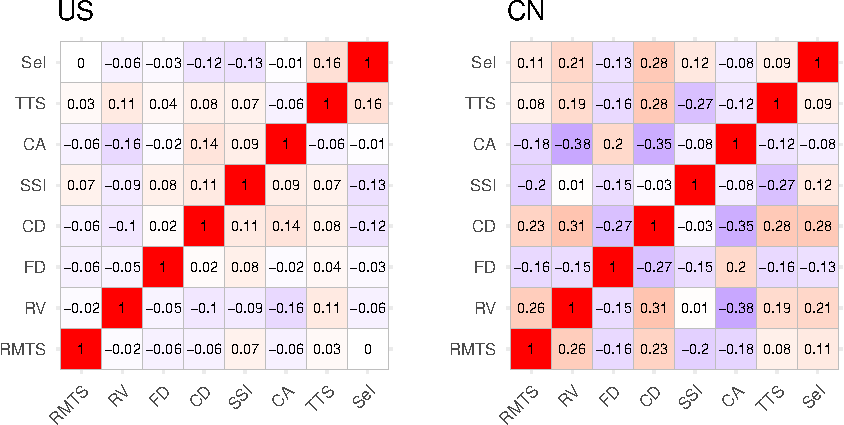
\includegraphics{CCRR_manuscript_files/figure-latex/unnamed-chunk-49-1.pdf}

\hypertarget{demographic-variation-in-responses}{%
\section{Demographic variation in responses}\label{demographic-variation-in-responses}}

In the exploratory analysis section, we explored how basic demographic variables could moderate the task performances within each culture. To do so, we fit an fixed effect model predicting each task's response in each culture, with each demographic variable as the predictor. We fit 192 exploratory regression models in total. 26 models were statistically significant, but only 1 survived Bonferroni correction. However, given that some of the demographic variables have been previously found to moderate task performance, we can treat this post-hoc exploratory analysis as a proxy for a conceptual replication. Therefore, we report selected uncorrected model results that are significant for key demographic variables in the tables below. These results should be interpreted with great cautions.

\hypertarget{residential-mobility}{%
\subsection{Residential Mobility}\label{residential-mobility}}

Higher residential mobility has been found to be related to individual's stronger emphasis on the independent self over the inter-dependent self (Ishii, Komiya, \& Oishi, 2020; Oishi \& Tsang, 2022). In our exploratory analysis's uncorrected models, residential mobility is a significant predictor to three task responses: U.S. participants' accuracy of Ebbinghaus Illusion task for U.S. participants, Chinese participants' proportion of first mention being focal objects in the Free Description task in Experiment 2, and U.S. participants' proportion of the taxonomic match selection in the Taxonomic-Thematic Similarity task. We reported the model results below.

\begin{table}[H]
\centering\begingroup\fontsize{9.5}{11.5}\selectfont

\begin{tabular}{l|l|l|r|r|r|r}
\hline
Study & Culture & Task Name & Beta & SE & t & p\\
\hline
Experiment 1 & US & Ebbinghaus Illusion & -0.01 & 0.01 & -2.01 & 0.05\\
Experiment 2 & CN & Free Description & 0.03 & 0.01 & 2.45 & 0.02\\
Experiment 2 & US & Taxonomic-Thematic Similarity & 0.01 & 0.00 & 2.59 & 0.01\\
\hline
\end{tabular}
\endgroup{}
\end{table}

\hypertarget{socioeconomic-status}{%
\subsection{Socioeconomic Status}\label{socioeconomic-status}}

\hypertarget{macarthur-ladder}{%
\subsubsection{MacArthur Ladder}\label{macarthur-ladder}}

The MacAuthur ladder scale is a subjective measure of socioeconomic status (Adler et al., 2000). This measurement has been found to show moderate relationship with the objective socioeconomic measurements, and it has even more robust relationship to individual's subjective well beings than objective socioeconomic measurements (J. J. Tan, Kraus, Carpenter, \& Adler, 2020). Past work has used this measure to investigate the relationship between socioeconomic status and individual's independent versus interdependent orientation (e.g., Miyamoto et al., 2018). In our current study, this measure was a significant predictor for five different tasks across two studies. In experiment 1, MacArthur Ladder scale response was negatively correlated with the proportion of participants choosing the unique pen in the U.S. participants. In experiment 2, this measure is negatively associated with the relational match Chinese participants selected in the Causal RMTS task, the score U.S. participants received in the Raven's Progressive Matrices, Chinese participants' reaction time in the Change Detection task, and the proportion of taxonomic-match Chinese participants selected in the Taxonomic-Thematic Similarity task. Theses results were summarized in the table below.

\begin{table}[H]
\centering\begingroup\fontsize{9.5}{11.5}\selectfont

\begin{tabular}{l|l|l|r|r|r|l}
\hline
Study & Culture & Task Name & Beta & SE & t & p\\
\hline
Experiment 1 & US & Uniqueness Preference & -0.05 & 0.02 & -2.36 & 0.02\\
Experiment 2 & CN & Causal RMTS & -0.04 & 0.02 & -2.05 & 0.04\\
Experiment 2 & US & Raven's Progressive Matrices & -0.02 & 0.01 & -2.14 & 0.03\\
Experiment 2 & CN & Change Detection & -735.86 & 221.15 & -3.33 & < .001\\
Experiment 2 & CN & Taxonomic-Thematic Similarity & -0.03 & 0.01 & -2.05 & 0.04\\
\hline
\end{tabular}
\endgroup{}
\end{table}

\hypertarget{maternal-education}{%
\subsubsection{Maternal Education}\label{maternal-education}}

Maternal education is often regarded as a proxy for socioeconomic status (Hauser, 1994; Hoff \& Tian, 2005). In the exploratory analysis, we first treated maternal education as a continuous variable. There was only one significant result: Chinese participants reported having higher maternal education made less situational attribution in the Causal Attribution task. Following common practices in the literature, we also binned the maternal education into a binary variable -- whether participants have received college education or not. The binary variable was not significantly related to any task performance.

\begin{table}[H]
\centering\begingroup\fontsize{9.5}{11.5}\selectfont

\begin{tabular}{l|l|l|r|r|r|r}
\hline
Study & Culture & Task Name & Beta & SE & t & p\\
\hline
Experiment 1 & CN & Causal Attribution & -0.08 & 0.04 & -2.22 & 0.03\\
\hline
\end{tabular}
\endgroup{}
\end{table}

\hypertarget{examples-of-tasks}{%
\section{Examples of Tasks}\label{examples-of-tasks}}

\hypertarget{experiment-1-2}{%
\subsection{Experiment 1}\label{experiment-1-2}}

\hypertarget{ambiguous-relational-match-to-sample-crmts}{%
\subsubsection{Ambiguous Relational Match-To-Sample (cRMTS)}\label{ambiguous-relational-match-to-sample-crmts}}

In the ambiguous cRMTS task (Carstensen et al., 2019, Experiment 3), participants were shown two pairs of objects, AB (A: blue square in the example setup shown in Figure \ref{fig:crmts-example}; B: yellow circle) and AC (C: red triangle), activating a music machine during the training phase. In the test phase, they were given a forced choice between an object-based solution (a \emph{same} pair of object A, i.e., a pair of blue squared in the example) and a relational solution (a \emph{different} pair BC, i.e., yellow circle and red triangle in the example).

\begin{figure}[H]

{\centering 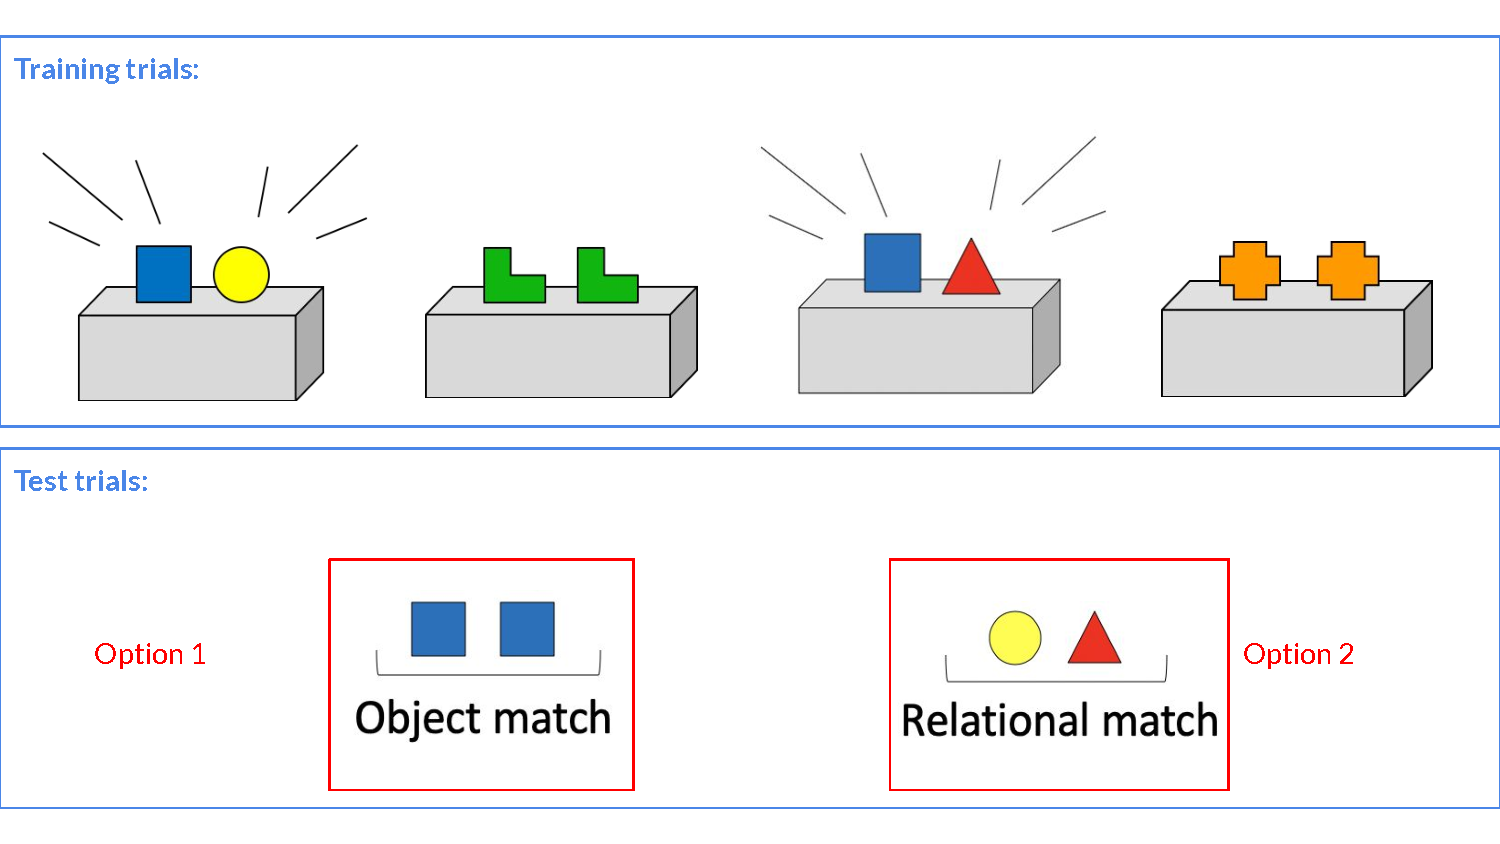
\includegraphics[width=1\linewidth,height=200px]{CCRR_manuscript_files/appendix_task_examples/e1_crmts} 

}

\caption{Ambiguous relational match-to-sample (cRMTS) task. Participants were given a forced choice between object-based solution (Option 1) and relational solution (Option 2) during the test phase.}\label{fig:crmts-example}
\end{figure}

\hypertarget{picture-free-description-2}{%
\subsubsection{Picture Free Description}\label{picture-free-description-2}}

In the picture free description task (Imada et al., 2013), Participants were shown a series of images with focal and background objects. For each image, they were asked to study it for 5 seconds, and then typed a description for it from memory.

\begin{figure}[H]

{\centering 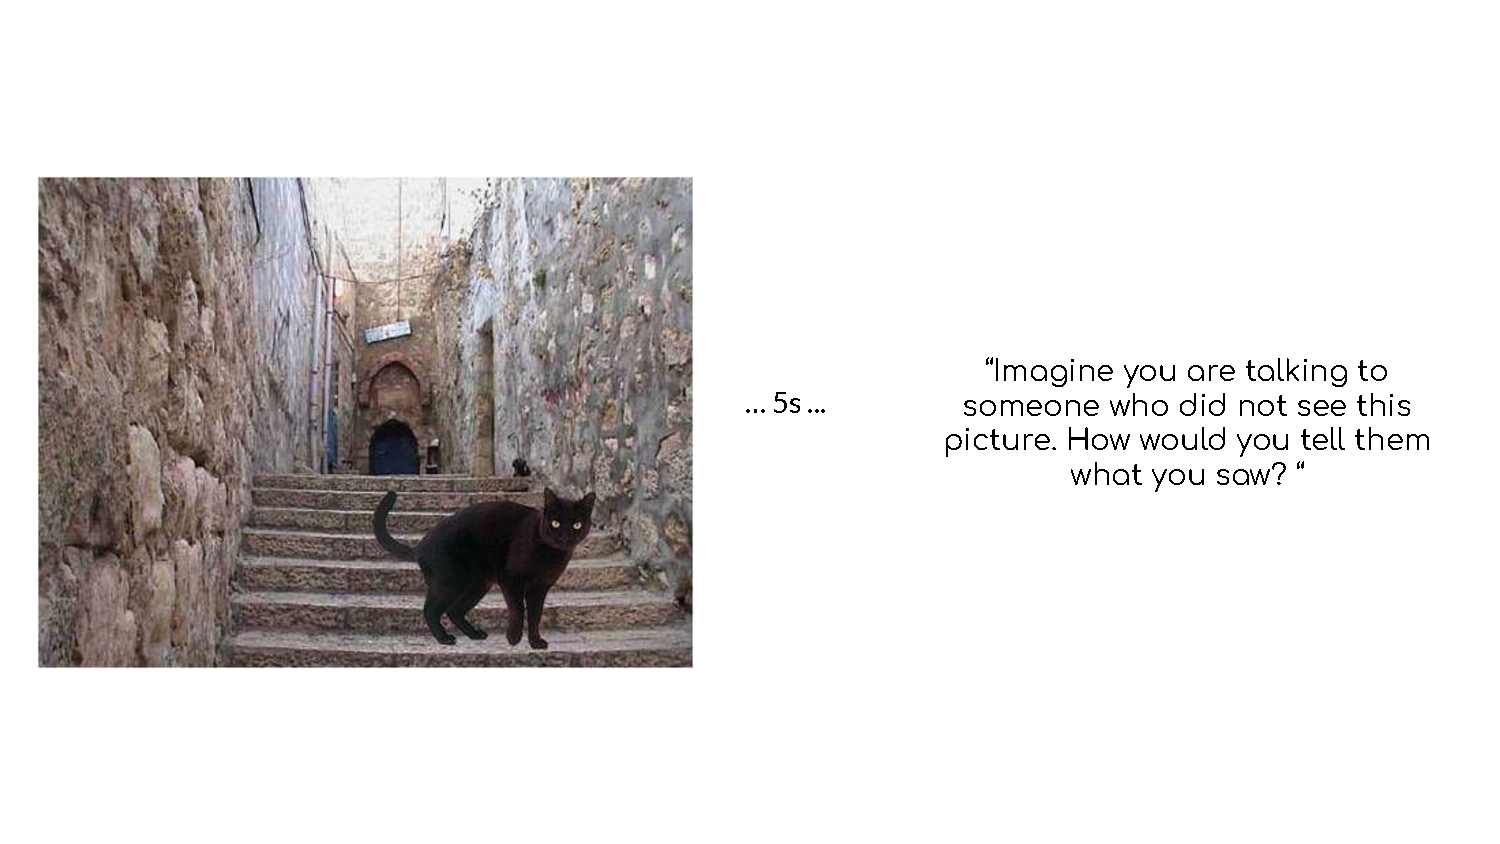
\includegraphics[width=1\linewidth,height=200px]{CCRR_manuscript_files/appendix_task_examples/e1_fd} 

}

\caption{A practice trial in picture free description task. In this image, the cat is the focal object, and the rest are background objects.}\label{fig:free-description}
\end{figure}

\hypertarget{ebbinghaus-illusion-1}{%
\subsubsection{Ebbinghaus Illusion}\label{ebbinghaus-illusion-1}}

In the Ebbinghaus illusion task (Imada et al., 2013), participants were asked to indicate which of the two orange circles (see Figure \ref{fig:ebbinghaus}) was larger. They completed the task in two blocks: (1) no context block (upper right panel), where the two orange circles appeared independently; (2) illusional context block (bottom right panel), where each of the two orange circles were flanked by a grid of 8 gray circles which are all smaller or larger than the center orange circle.

\begin{figure}[H]

{\centering 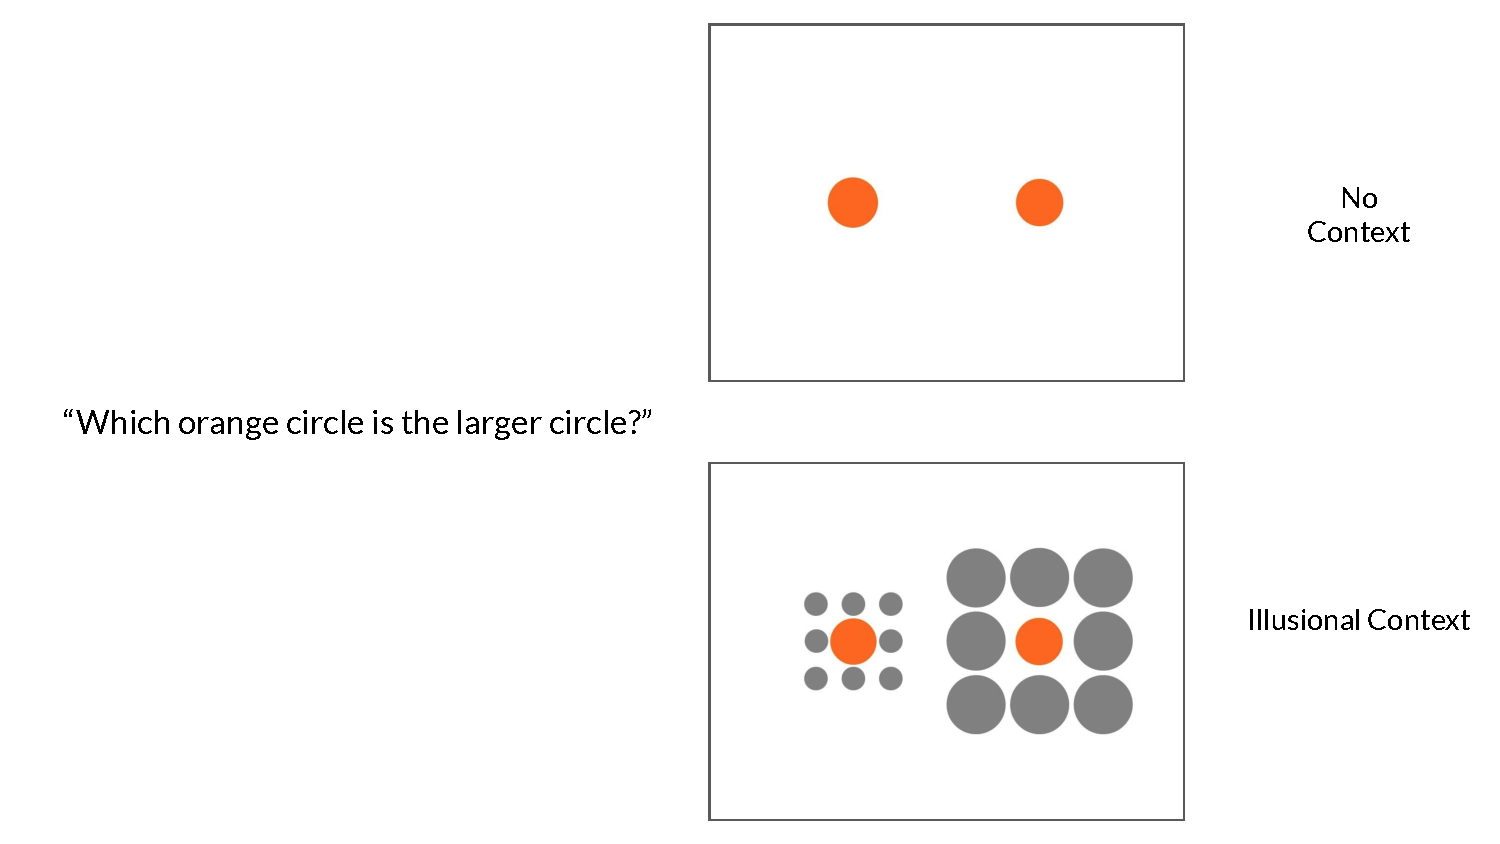
\includegraphics[width=1\linewidth,height=200px]{CCRR_manuscript_files/appendix_task_examples/e1_ebbinghaus} 

}

\caption{Ebbinghaus illusion task. Upper right panel: no context block. Bottom right panel: illusional context block.}\label{fig:ebbinghaus}
\end{figure}

\hypertarget{horizon-collage-2}{%
\subsubsection{Horizon Collage}\label{horizon-collage-2}}

In the horizon collage task (Senzaki et al., 2014), participants were asked to create ``a picture of the outside'' by dragging-and-dropping sticker objects onto a rectangular ``canvas.'' They were told to include a horizon line and could use any number of other stickers to create their image.

\begin{figure}[H]

{\centering 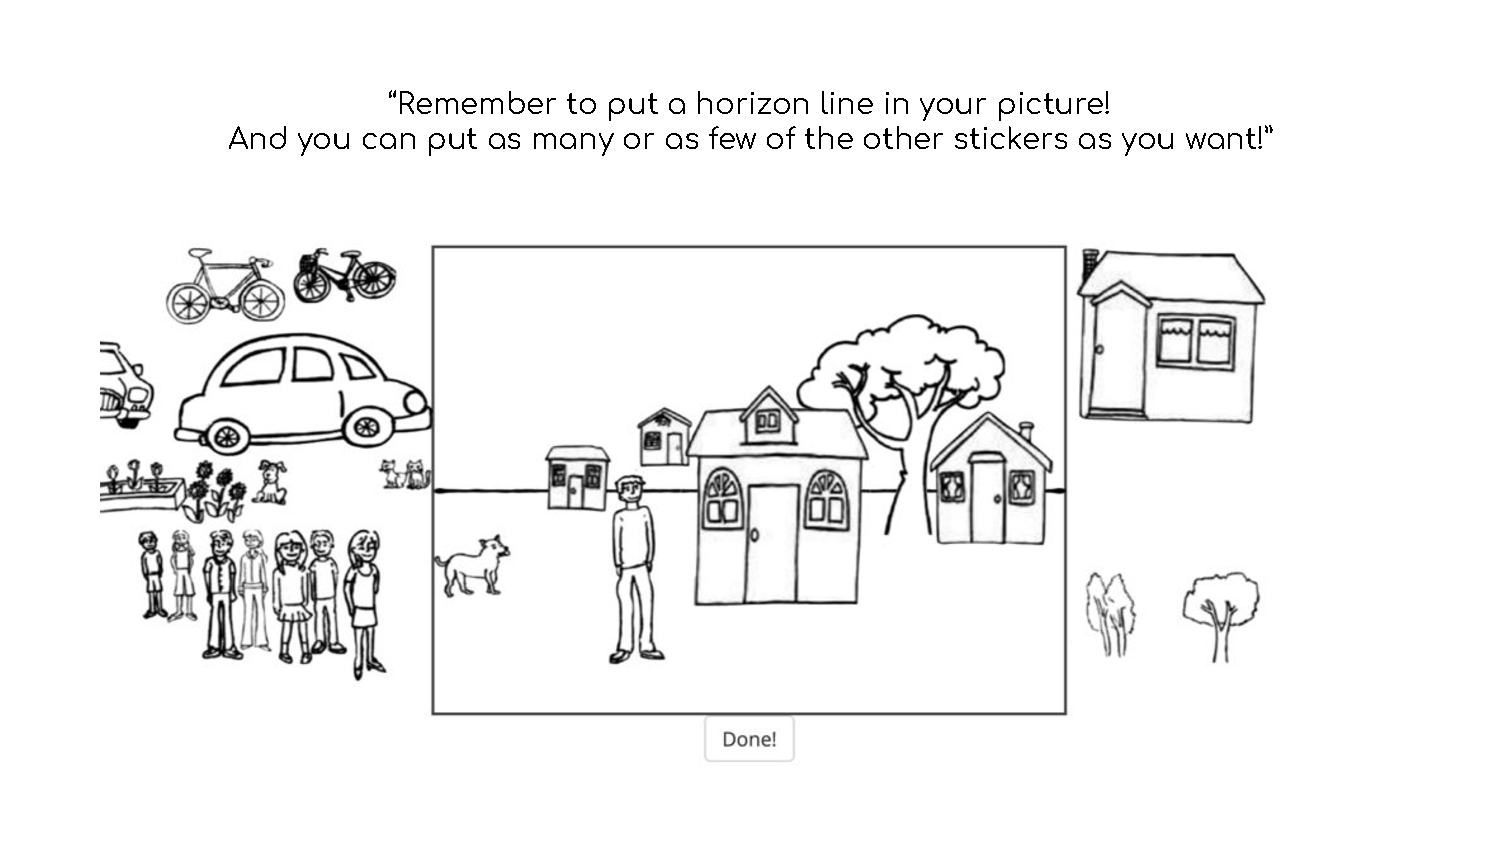
\includegraphics[width=1\linewidth,height=200px]{CCRR_manuscript_files/appendix_task_examples/e1_horizon} 

}

\caption{Horizon collage task. Participants created an image of the outside by dragging-and-dropping sticker objects onto a rectangular "canvas."}\label{fig:horizon}
\end{figure}

\hypertarget{symbolic-self-inflation-family}{%
\subsubsection{Symbolic Self-Inflation (Family)}\label{symbolic-self-inflation-family}}

In the adapted symbolic self-inflation task (Kitayama et al., 2009), we asked participants to draw themselves and their family members as circles by clicking-and-dragging their mouse on a rectangular ``canvas.''

\begin{figure}[H]

{\centering 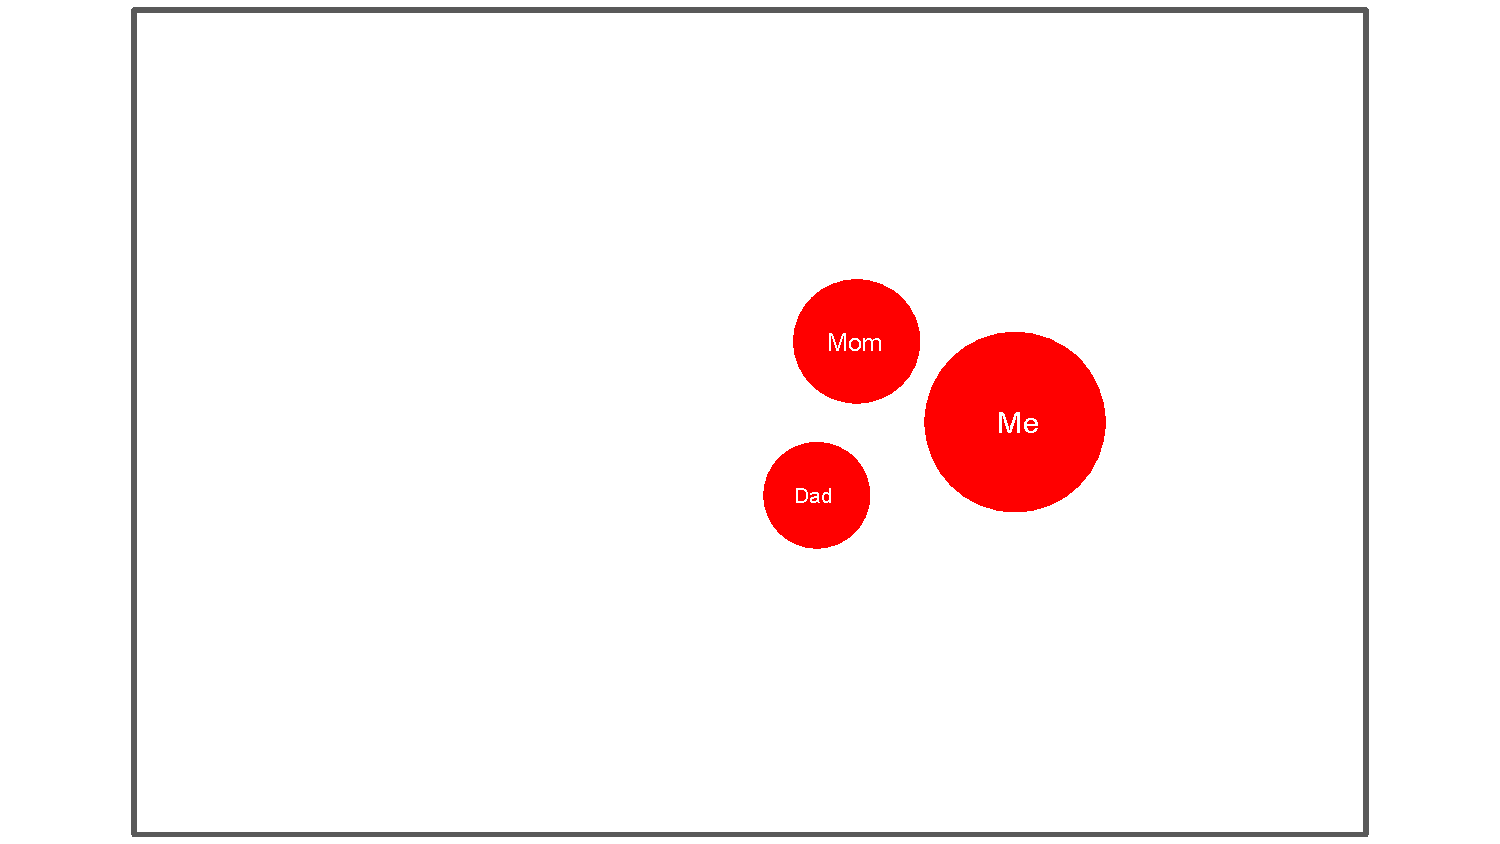
\includegraphics[width=1\linewidth,height=200px]{CCRR_manuscript_files/appendix_task_examples/e1_si_family} 

}

\caption{Symbolic self-inflation task, family version. In this example, three circles were drawn representing the participant, their mother, and their father, respectively.}\label{fig:si-family}
\end{figure}

\hypertarget{uniqueness-preference-1}{%
\subsubsection{Uniqueness Preference}\label{uniqueness-preference-1}}

In this adapted version of the uniqueness preference task (Kim \& Markus, 1999), participants were asked to select one of the five dinosaur ``stickers'' that were identical except for color (four blue and one yellow).

\begin{figure}[H]

{\centering 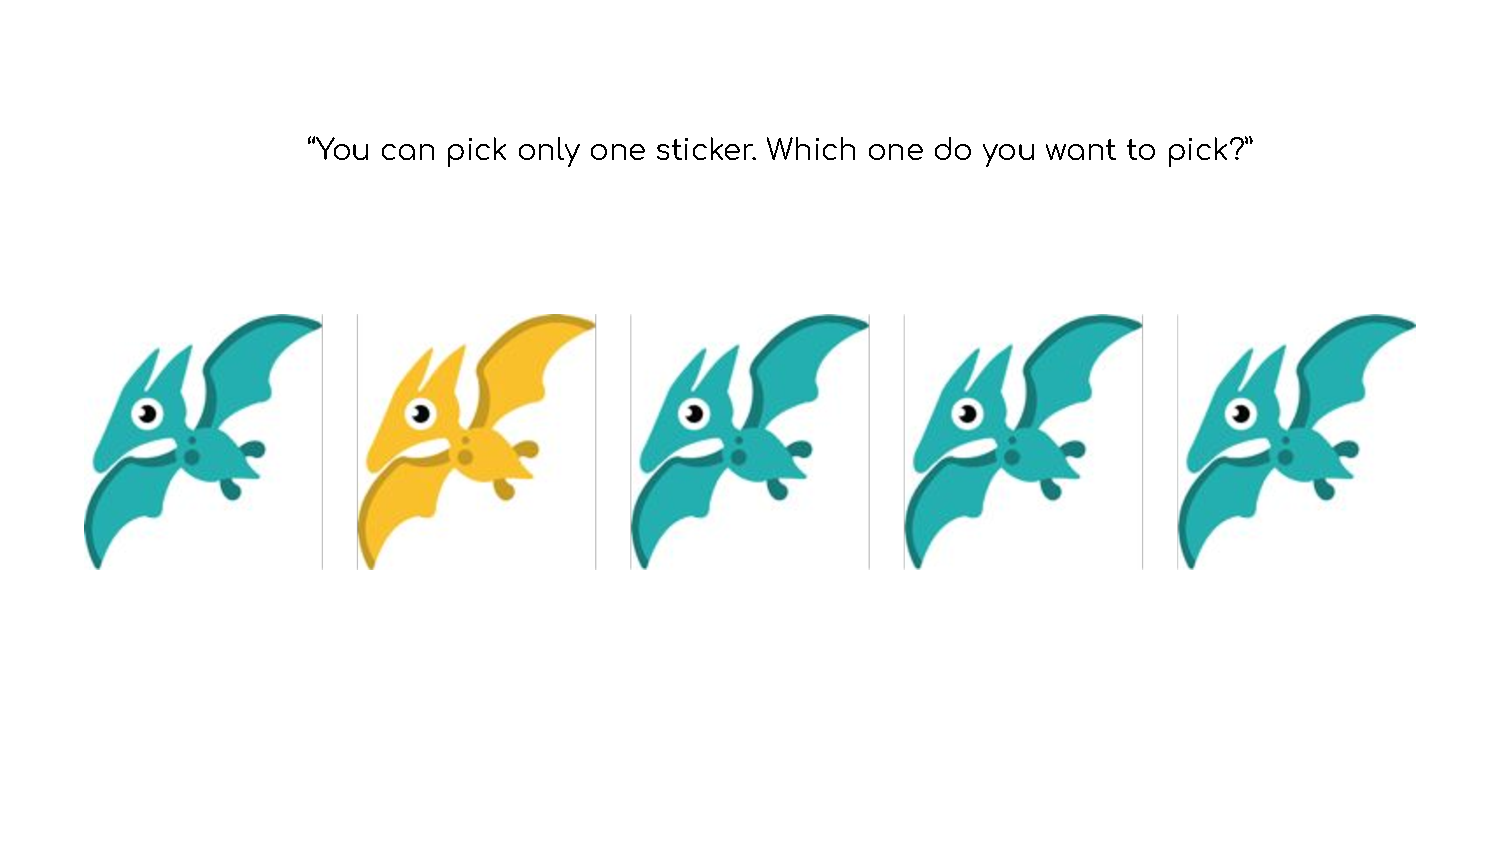
\includegraphics[width=1\linewidth,height=200px]{CCRR_manuscript_files/appendix_task_examples/e1_uniqueness} 

}

\caption{Uniqueness preference task. Participants were asked to select one of the five dinosaur "stickers."}\label{fig:uniqueness}
\end{figure}

\hypertarget{child-causal-attribution-1}{%
\subsubsection{Child Causal Attribution}\label{child-causal-attribution-1}}

In the child causal attribution task (Seiver et al., 2013), participants watched a series of four short, animated vignettes in which two children both played in a pool and neither child played on a bicycle. They were then asked to explain in text why each child did not play on the bicycle.

\begin{figure}[H]

{\centering 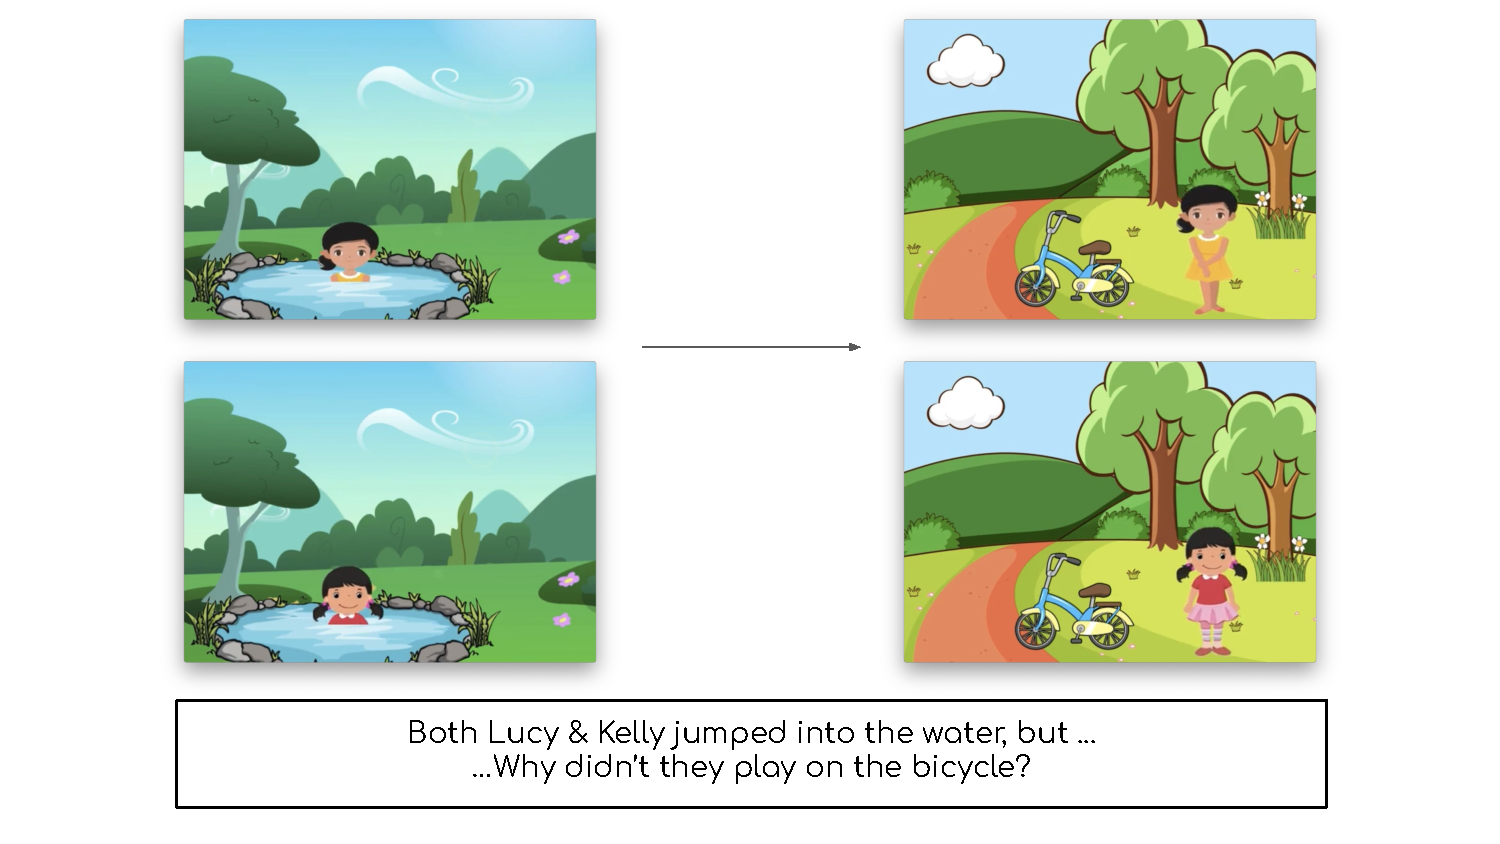
\includegraphics[width=1\linewidth,height=200px]{CCRR_manuscript_files/appendix_task_examples/e1_ca_child} 

}

\caption{Child causal attribution task. Participants were asked to explain why each child did not play on the bicycle}\label{fig:ca-child}
\end{figure}

\hypertarget{ravens-standard-progressive-matrices-2}{%
\subsubsection{Raven's Standard Progressive Matrices}\label{ravens-standard-progressive-matrices-2}}

In Raven's standard progressive matrices task, participants were asked to select from a series of given options one that best completed the patterns demonstrated in the prompts.

\begin{figure}[H]

{\centering 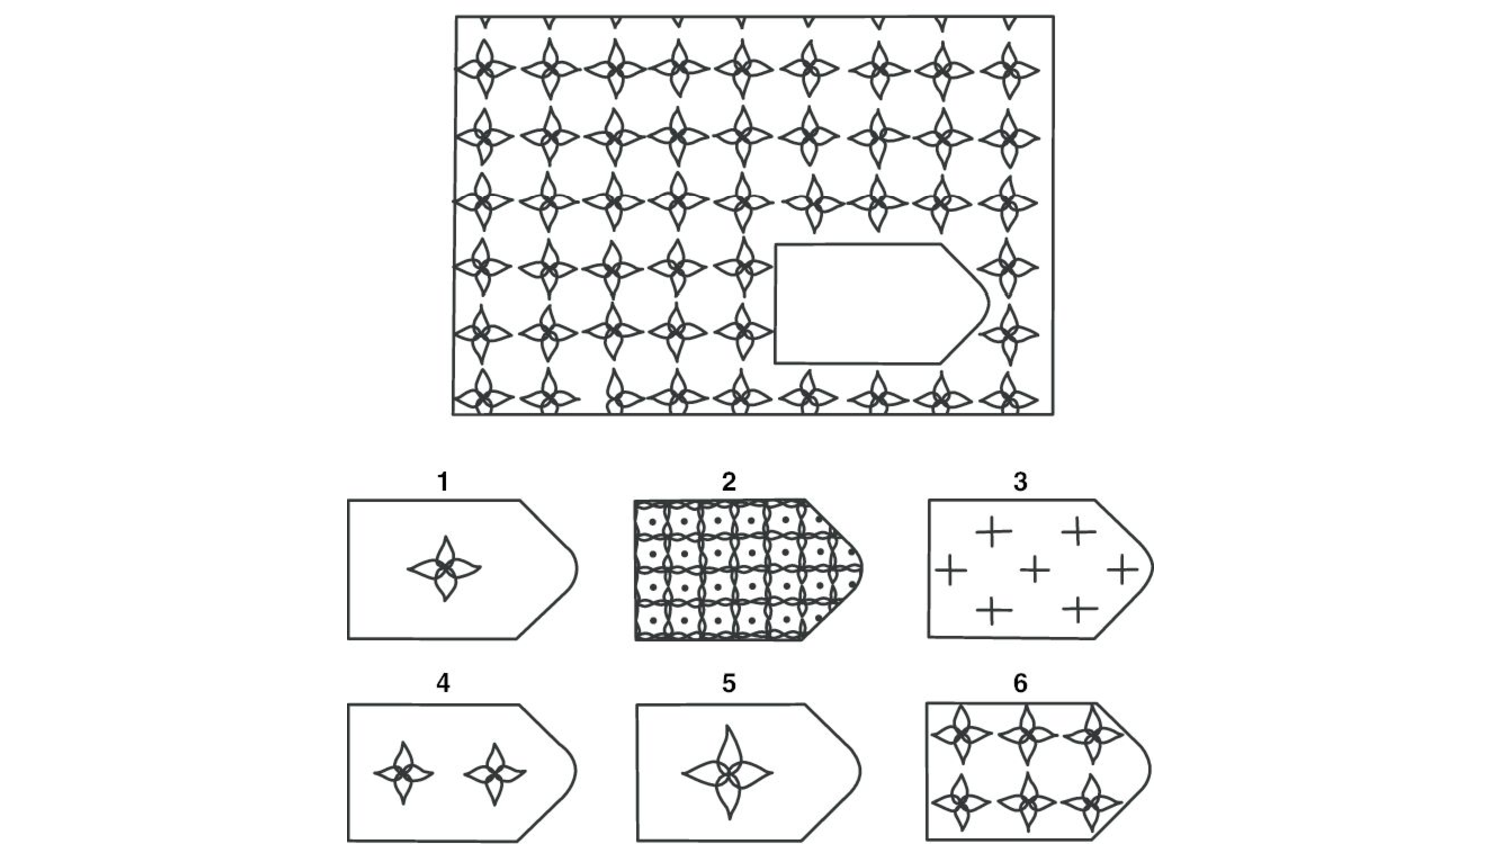
\includegraphics[width=1\linewidth,height=200px]{CCRR_manuscript_files/appendix_task_examples/e1_raven} 

}

\caption{Raven's standard progressive matrices task. Participants were asked to select one option that best completed the patterns demonstrated in the prompts (upper panel).}\label{fig:raven}
\end{figure}

\hypertarget{experiment-2-2}{%
\subsection{Experiment 2}\label{experiment-2-2}}

In Experiment 2, the following tasks followed the same procedures as in Experiment 1: ambiguous relational match-to-sample (ambiguous cRMTS), picture free description, and Raven's progressive matrices. The symbolic self-inflation task also followed similar procedures as in Experiment 1, except that participants were told to draw themselves and their \emph{friends} into circles this time, as opposed to drawing draw themselves and their \emph{family members} into circles in Experiment 1. We show examples for the remaining four tasks in Experiment 2 below.

\hypertarget{adult-causal-attribution-2}{%
\subsubsection{Adult Causal Attribution}\label{adult-causal-attribution-2}}

In the adult version causal attribution task (Morris \& Peng, 1994), participants were randomly assigned to read one of two crime stories (Royal Oak shooting or Iowa shooting). They were then asked to write a short explanation for the murderer's behaviors and rate a list of statements about the causes of the murder (attributing to personal or situational factors) on a 7-point Likert scale.

\begin{figure}[H]

{\centering 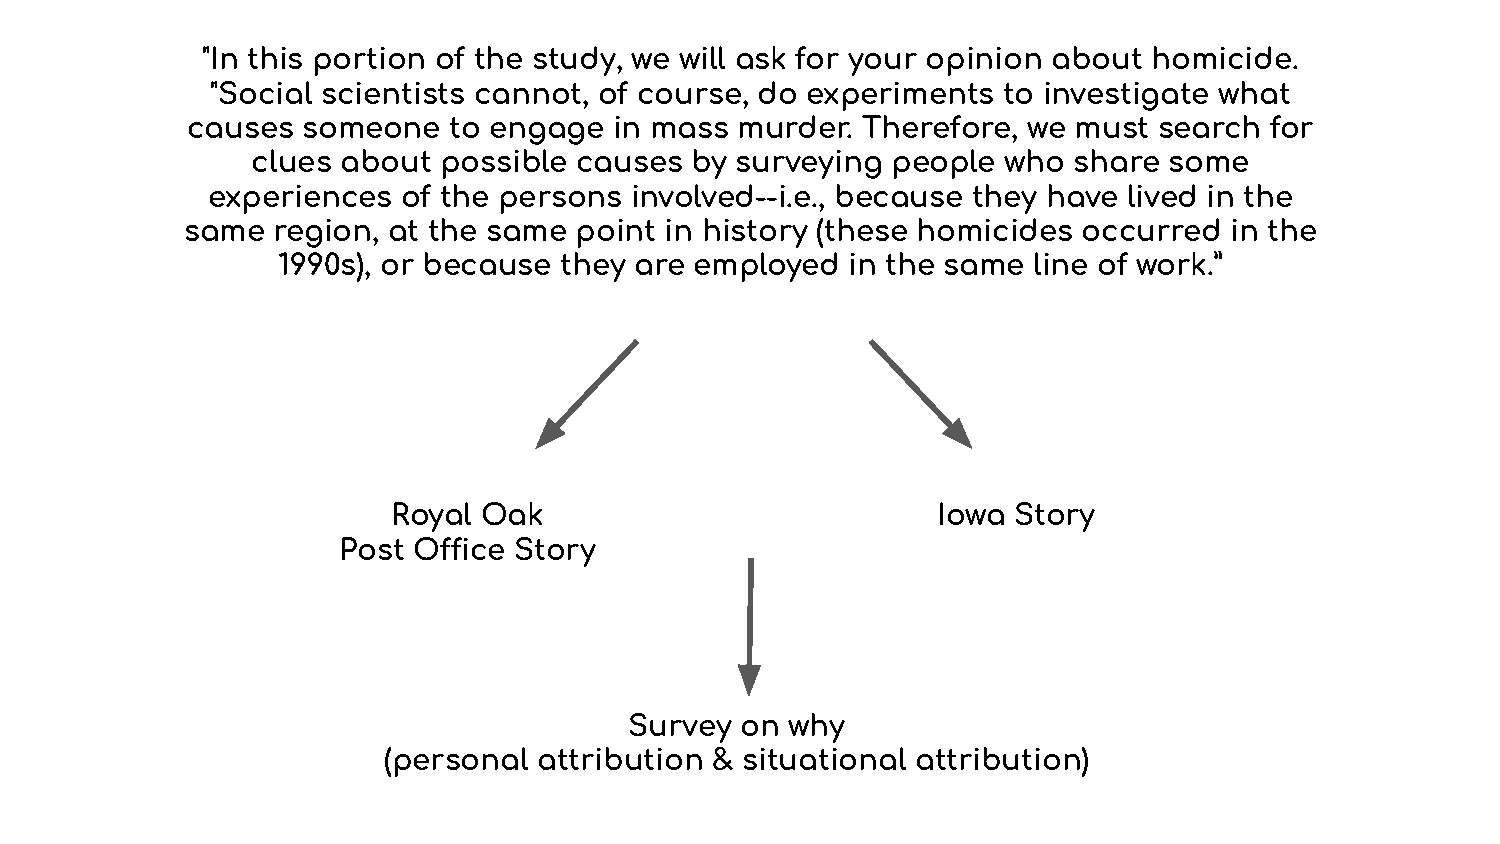
\includegraphics[width=1\linewidth,height=200px]{CCRR_manuscript_files/appendix_task_examples/e2_ca_adult} 

}

\caption{Adult causal attribution task. Participants were randomly assiged to read one of two crime stories (Royal Oak shooting or Iowa shooting) and make attributions for the murder.}\label{fig:ca-adult}
\end{figure}

\hypertarget{change-detection-2}{%
\subsubsection{Change Detection}\label{change-detection-2}}

In each trial of the change detection task (Masuda \& Nisbett, 2006), a pair of images would alternate on the screen, each presented for 560ms with a blank screen in between images for 80ms. The two pictures were almost identical with subtle differences, either in the focal object (e.g., a tractor with or without a wheel, as shown in the left panel of Figure \ref{fig:change-detection}) or the background (e.g., a scaffold in the distance with varying size, as shown in the right panel of Figure \ref{fig:change-detection}). Participants were instructed to press a key when they spotted the difference, and then describe the difference in a text box. If they did not detect a difference within 60 seconds, the trial timed out.

\begin{figure}[H]

{\centering 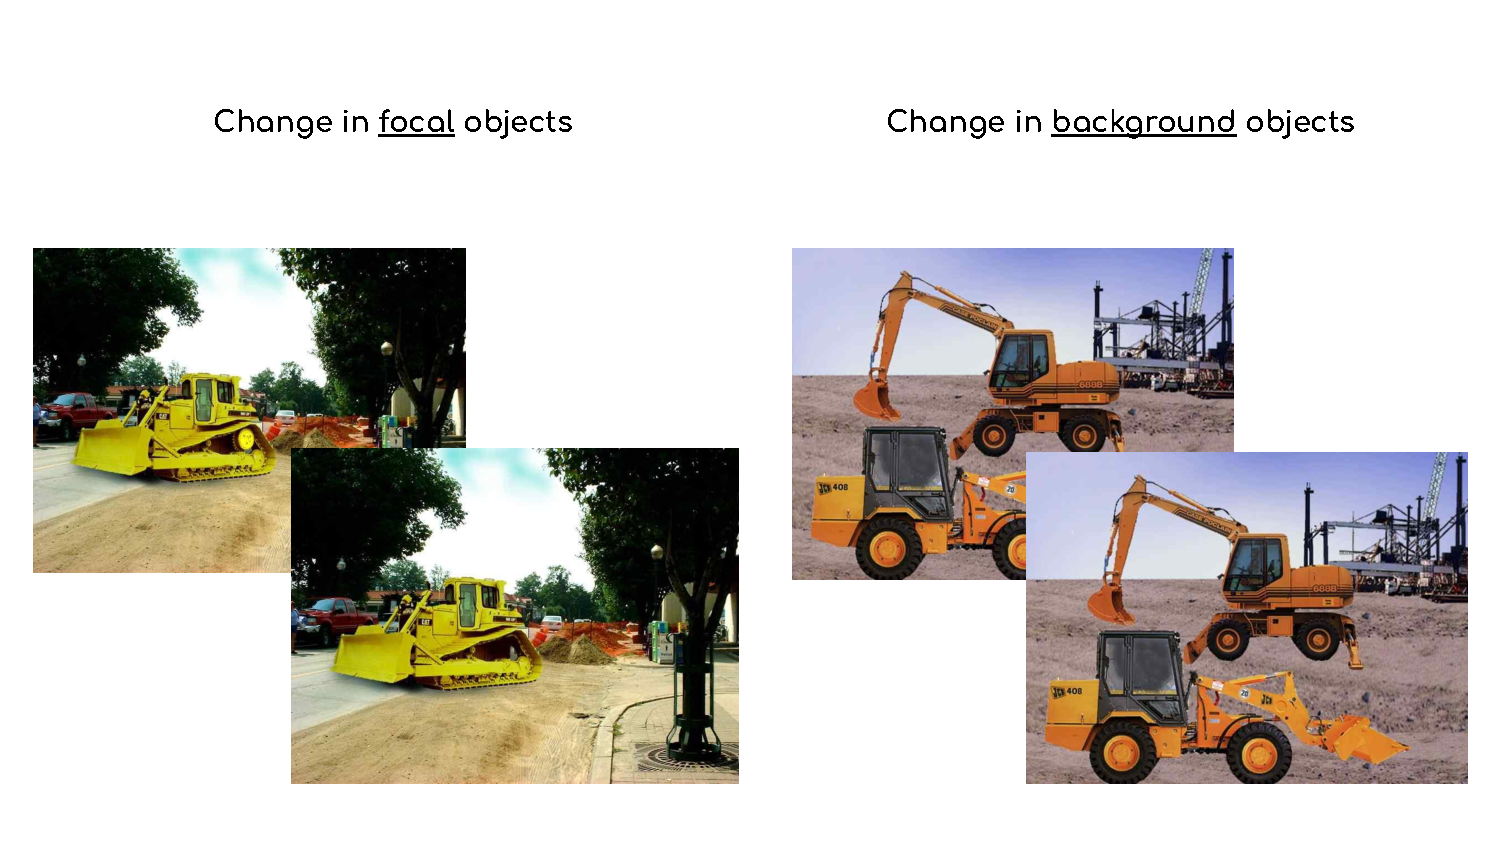
\includegraphics[width=1\linewidth,height=200px]{CCRR_manuscript_files/appendix_task_examples/e2_cd} 

}

\caption{Change detection task. Participants were instructed to detect the difference in each pair of images as quickly as they could. Left panel: change happened in a focal object. Right panel: change happened in the background.}\label{fig:change-detection}
\end{figure}

\hypertarget{taxonomic-thematic-similarity-2}{%
\subsubsection{Taxonomic-Thematic Similarity}\label{taxonomic-thematic-similarity-2}}

In the taxonomic-thematic similarity task (Ji et al., 2004; Le et al., 2021), participants were presented with triads containing a cue word and two match options. In each test triad (as shown in Figure \ref{fig:similarity}), one option was a taxonomic match (e.g., ladybug and bee are both insects) and the other a thematic match (e.g., bees usually appear in gardens). In each filler triads, the cue item and the options were broadly similar, thematically and taxonomically, making for a more ambiguous decision (e.g., monkey: elephant, tiger). Participants completed a two-alternative forced choice task in which they chose one match for each cue item.

\begin{figure}[H]

{\centering 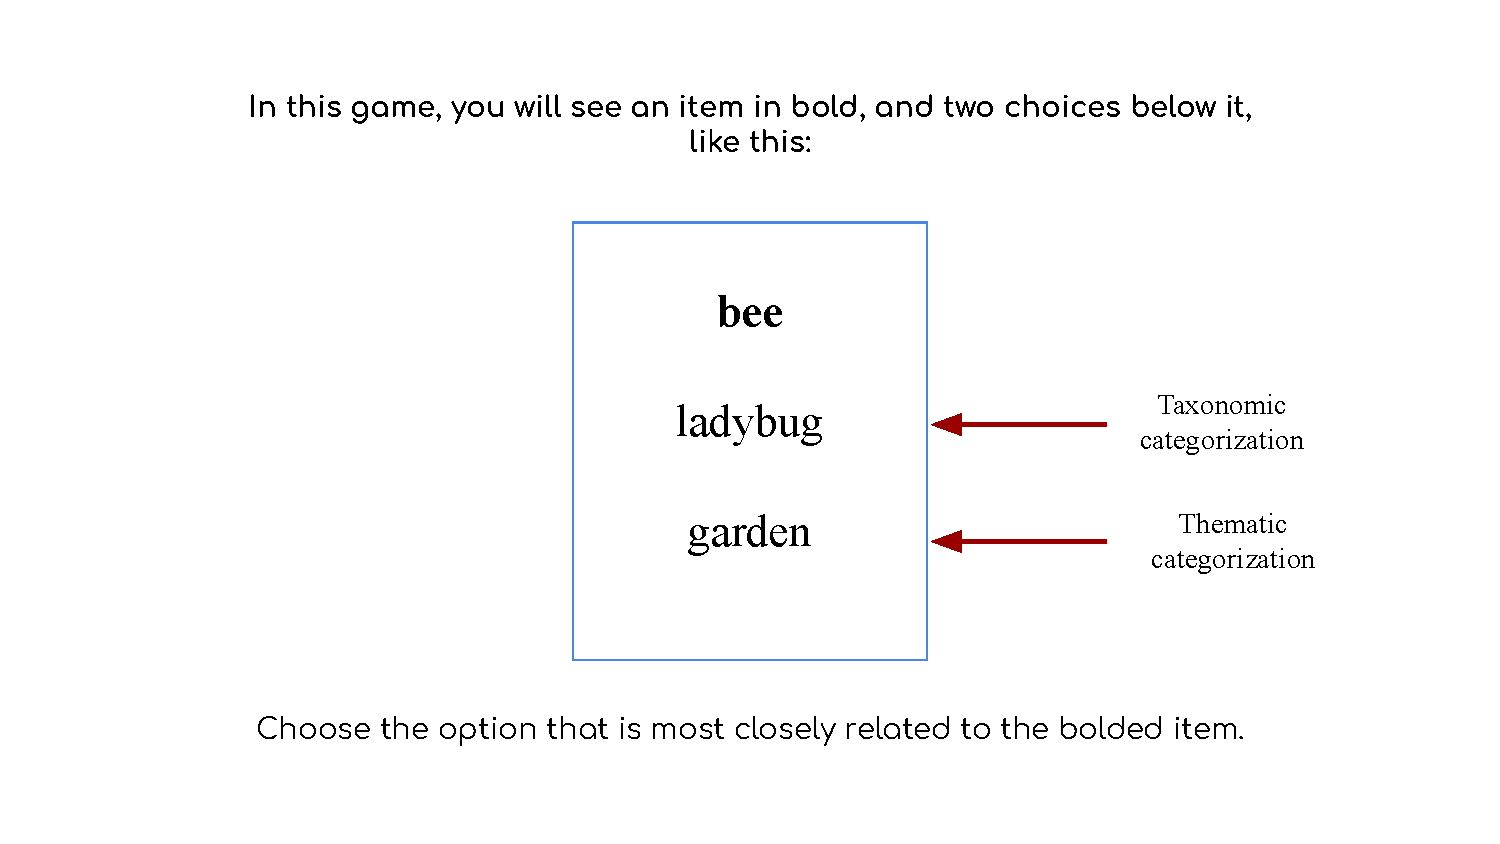
\includegraphics[width=1\linewidth,height=200px]{CCRR_manuscript_files/appendix_task_examples/e2_similarity} 

}

\caption{Taxonomic-thematic similarity task. Participants completed a two-alternative forced choice task in which they chose one match for each cue item.}\label{fig:similarity}
\end{figure}

\hypertarget{semantic-intuition-2}{%
\subsubsection{Semantic Intuition}\label{semantic-intuition-2}}

In the semantic intuition task (Li et al., 2018), participants read five stories and judged the correctness of statements referring to a character after each story. The correctness judgement reflected their semantic intuition of either the descriptivist view (i.e., determine the referent of a name based on the description of the speaker) or the causal-historical view (i.e., determine the referent based on the original usage).

\begin{figure}[H]

{\centering 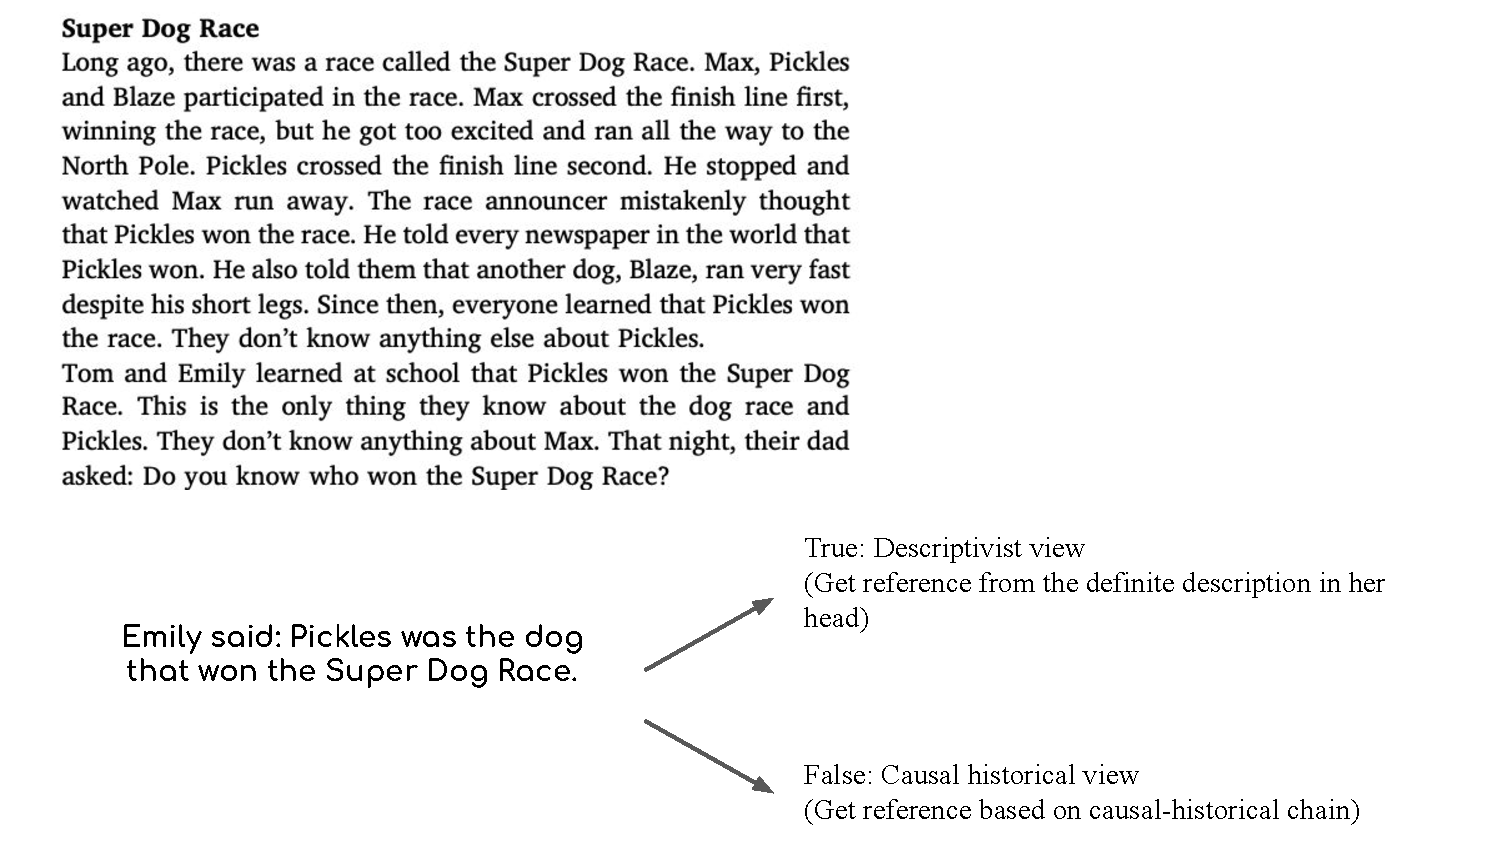
\includegraphics[width=1\linewidth,height=200px]{CCRR_manuscript_files/appendix_task_examples/e2_semantic} 

}

\caption{Semantic intuition task. In this specific example, judging the statement as "true" indicates a descriptivist view, and judging it as "false" indicates a causal-historical view.}\label{fig:semantic}
\end{figure}


\end{document}
